% !TeX program = pdfLaTeX
\documentclass[12pt]{article}
\usepackage{amsmath}
\usepackage{graphicx,psfrag,epsf}
\usepackage{enumerate}
\usepackage{natbib}
\usepackage{textcomp}
\usepackage[hyphens]{url} % not crucial - just used below for the URL
\usepackage{hyperref}
\usepackage{listings}
\usepackage[usenames,dvipsnames]{color}    

\lstset{ 
  language=R,                     % the language of the code
  basicstyle=\scriptsize\ttfamily,      % the size of the fonts that are used for the code
  numbers=left,                   % where to put the line-numbers
  numberstyle=\scriptsize\color{Blue},  % the style that is used for the line-numbers
  stepnumber=1,                   % the step between two line-numbers. If it is 1, each line
                                  % will be numbered
  numbersep=5pt,                  % how far the line-numbers are from the code
  backgroundcolor=\color{white},  % choose the background color. You must add \usepackage{color}
  showspaces=false,               % show spaces adding particular underscores
  showstringspaces=false,         % underline spaces within strings
  showtabs=false,                 % show tabs within strings adding particular underscores
  frame=single,                   % adds a frame around the code
  rulecolor=\color{black},        % if not set, the frame-color may be changed on line-breaks within not-black text (e.g. commens (green here))
  tabsize=2,                      % sets default tabsize to 2 spaces
  captionpos=b,                   % sets the caption-position to bottom
  breaklines=true,                % sets automatic line breaking
  breakatwhitespace=false,        % sets if automatic breaks should only happen at whitespace
  keywordstyle=\color{RoyalBlue},      % keyword style
  commentstyle=\color{YellowGreen},   % comment style
  stringstyle=\color{ForestGreen}      % string literal style
}
 
\providecommand{\tightlist}{%
  \setlength{\itemsep}{0pt}\setlength{\parskip}{0pt}}

%\pdfminorversion=4
% NOTE: To produce blinded version, replace "0" with "1" below.
\newcommand{\blind}{0}

% DON'T change margins - should be 1 inch all around.
\addtolength{\oddsidemargin}{-.5in}%
\addtolength{\evensidemargin}{-.5in}%
\addtolength{\textwidth}{1in}%
\addtolength{\textheight}{1.3in}%
\addtolength{\topmargin}{-.8in}%

%% load any required packages here

\makeatletter
\newcommand*{\centerfloat}{%
  \parindent \z@
  \leftskip \z@ \@plus 1fil \@minus \textwidth
  \rightskip\leftskip
  \parfillskip \z@skip}
\makeatother

\begin{document}

\def\spacingset#1{\renewcommand{\baselinestretch}%
{#1}\small\normalsize} \spacingset{1}

%%%%%%%%%%%%%%%%%%%%%%%%%%%%%%%%%%%%%%%%%%%%%%%%%%%%%%%%%%%%%%%%%%%%%%%%%%%%%%

\if0\blind
{
  \title{\bf Statistical Methods for Accounting Systems}

  \author{
        Stijn Masschelein \thanks{The authors are grateful for comments by seminar participants at Australian National University, Leuven University, the 2018 AFAANZ conference, and the 2018 AOS conference on Management Control as System or Package in Maastricht.} \\
    University of Western Australia Business School\\
     and \\     Frank Moers \\
    Maastricht University School of Business and Economics\\
      }
  \maketitle
} \fi

\if1\blind
{
  \bigskip
  \bigskip
  \bigskip
  \begin{center}
    {\LARGE\bf Statistical Methods for Accounting Systems}
  \end{center}
  \medskip
} \fi

\bigskip
\begin{abstract}
Following the theoretical innovations of complementarity theory, management control studies have investigated potential interdependencies between management control practices. In this paper, we compare the two dominant statistical specifications to test for the presence of interdependencies. While prior literature focuses on the assumption of optimality when deciding between the demand specification and the performance specification, we make all ancillary assumptions explicit. Our simulation results reveal that the demand specification is more robust to variations in optimality and correlated omitted variables than the performance specification. We use these results to formulate guidance for future research into management control interdependencies.
\end{abstract}

\noindent%
{\it Keywords:} Complementarity Theory, Management Control, Statistical Methods
\vfill

\newpage

\spacingset{1.15}

\section{Introduction}\label{introduction}

 Complementarity theory posits that interdependent management control practices can be seen as one coherent management control system \citep{milgrom_complementarities_1995, grabner_management_2013}. Different streams of literature have investigated such interdependencies between management control practices. For instance, agency theory argues that incentive design and delegation of decision rights are complements \citep{holmstrom_firm_1994}. The management accounting literature has established that at least under certain conditions, delegation of decision rights to managers complements incentive contracts \citep{bouwens_assessing_2007, indjejikian_accounting_2012, moers_performance_2006}. Drawing on the original work by \citet{simons_levers_1994, simons_performance_2000}, the levers of control literature has investigated potential complementarities between the four levers \citep{widener_empirical_2007}. Lastly, the budgeting literature has long argued that the effectiveness of budget participation depends on the the extent to which the budget is used to evaluate employees \citep{brownell_task_1991, dunk_effect_1993}.
 
This paper compares the two main specifications to empirically test whether practices are complements: the performance specification and the demand specification \citep{grabner_management_2013}. The demand approach assumes that firms simultaneously choose the optimal level of the practices taking into account the interdependency and the firm's environment. Under this assumption, complementary practices are positively correlated with each other after controlling for environmental factors \citep{arora_testing_1996, grabner_management_2013, johansson_testing_2018, hofmann_organizational_2017}. For instance, delegation and accounting based incentives are expected to be correlated after controlling for contingency factors. In contrast, the performance specification assumes that there are a sufficient number of firms that deviate from those optimal choices which allows researchers to detect performance differences between optimal and suboptimal accounting systems. Under this assumption, the interaction between the two practices is positively correlated with performance \citep{athey_empirical_1998, carree_note_2011, grabner_management_2013, hofmann_organizational_2017}. For instance, the interaction between delegation and accounting based incentives is positively related to business unit performance. 

In observational samples neither the assumption of completely randomly determined practices or the assumption of completely optimal choices will hold \citep{brynjolfsson_complementarity_2013}. The methodology literature has treated the assumption about the level of optimality in a sample as an untestable assumption and requires researchers to argue whether their chosen specification is appropriate for their research setting. \footnote{We refer to the overall distance between observed practices and the optimal levels in a sample as the \emph{level of optimality} of the sample. While an individual decision is either optimal or not, a sample of those individual decisions can exhibit different levels of optimality. That is, different samples can contain different proportions of optimal decisions.}
The demand specification is often seen as more appropriate than the performance specification when one decision maker has designed the entire accounting system, when the optimal design is not too complicated, and when the decision maker has had sufficient time and incentives to choose the optimal system \citep{grabner_management_2013, hofmann_organizational_2017, carree_note_2011, johansson_testing_2018}.  The performance specification is often deemed appropriate when there are a sufficient number of firms that do not adopt the optimal practices \citep{carree_note_2011, bedford_management_2016}. 

In this paper, we show how the demand and performance specification arise from the same underlying and unobserved objective function. The objective function formalises the performance effects of management accounting practices and how those performance effects depend on other practices and contingency factors. As such, the objective function captures the main insight of complementarity theory \citep{milgrom_complementarities_1995,grabner_management_2013} and contingency theory \citep{chenhall_management_2003,otley_contingency_2016}. We then show the statistical problems that arise with the demand and performance specification when their assumptions are not satisfied. First, the demand specification has more power to detect an interdependency when management control practices are closer to optimal while the performance specification is more likely to detect an interdependency when the control practices are further from optimal. Second, both specifications are vulnerable to the same omitted variable bias when they do not appropriately control for a contingency factor that affects both practices. The omitted variable problem is widely recognised for the demand specification \citep{grabner_management_2013, arora_testing_1996, hofmann_organizational_2017} but is largely ignored \citep{grabner_management_2013, hofmann_organizational_2017} or thought of as non-existing for the performance specification \citep{carree_note_2011}. We show how both specifications can control for the bias when all relevant practices and contingency factors are observed. Unfortunately, the most commonly used variant of the production specification does not address the bias.

Because the vulnerabilities of both specifications depend on the level of optimality in the empirical sample, we use a simulation to investigate the robustness of both specifications to variations in the level of optimality. The results show that the demand approach has appropriate type I error rates while maintaining power to detect a real complementary effect even at low levels of optimality. In contrast, the theoretically derived performance function approach suffers from elevated type I error rates at all levels of optimality and loses power to detect true interdependencies a higher levels of optimality. In addition, the performance specification as it is typically implemented is biased when the practices are contingent on the same environmental factor.

This study provides three recommendations for studies that test for interdependencies between management practices. First of all, the demand specification is generally preferred over the performance specification in an observational sample of firms. When performance data is available, it is still advisable to report the demand functions before reporting the performance specification \citep{aral_three-way_2012, cassiman_search_2006}. Second, when theory and prior research indicate that the practices are contingent on environmental factors, studies should appropriately control for these factors. Because the management control literature has a rich history of studying contingency effects, we believe most management control settings will warrant appropriate controls for environmental factors. In the demand specification, controlling for contingency factors means including the contingency variables as separate independent variables. In the performance specification, controlling for contingency effects requires including the interaction of the contingency factors with the management control practices. Of the published studies using the performance specification approach following \citet{grabner_management_2013}, only \citet{bedford_management_2016, bedford_performance_2019} appropriately control for contingency factors. Third, because the performance specification is vulnerable to Type I errors, we advise to use more robust estimation techniques than ordinary least squares.

The remainder of this paper is structured as follows. First, we derive the demand and performance specifications from a common objective function. Second, we explain and calibrate the simulation approach. Third, we compare the robustness of the different specifications in a simulation study. Fourth, we provide guidance for researchers who estimate interdependencies. Last, we summarise the simulation results and guidance, and discuss how future research can further the estimation of interdependencies.

\section{Model and formal analysis}\label{model-and-formal-analysis}

In this section, we present a firm's objective function that encapsulates the essential elements of both complementarity theory and contingency theory. Following complementarity theory, the performance of management control practices can depend on each other. Following contingency theory, the performance effects of the practices depend on the environment. The theoretical model helps to make the assumptions in the two statistical specifications explicit. We assume that a firm chooses the level of two management accounting practices which depend on one environmental factor. We represent the levels of the management accounting practices as vector $x_1$ and $x_2$ and the level of the environmental factors as a vector $z$. We further assume that the performance, $y$, depends on a the factor $\nu$ while the performance effects of each management control practices further depends on a factor $\epsilon_1$ and $\epsilon_2$ respectively. $x_1$, $x_2$ and $z$ are observed by the researcher but $\epsilon_1$, $\epsilon_2$, and $\nu$ are not. 

We apply the model to the management accounting literature where $z$ stands for environmental uncertainty, the most commonly studied environmental factor in the contingency literature. $x_1$ and $x_2$ are two commonly studied management control decisions, the extent to delegate decisions to middle level managers (henceforth delegation) and the extent to which accounting measures are used to evaluate and reward performance of the middle level managers (henceforth accounting incentives). Finally, $y$ is the financial performance of the business unit. These four constructs have received considerable attention in both the contingency and the complementarity literature \citep{grabner_management_2013,chenhall_management_2003, otley_contingency_2016}. In the example, we cannot do justice to the rich theories and measurement developed in the literature and therefore the example should only be seen as an illustration of the objective function.

\begin{equation}\label{eq:objective}
y  = \beta_0 + (\beta_{11} + \gamma_1 z + \epsilon_1) x_1 
						+ (\beta_{22} + \gamma_2 z  + \epsilon_2) x_2 
                        + \beta_{12} x_1 x_2 - \frac{1}{2}\delta_1 x^2_1 - \frac{1}{2}\delta_2 x^2_2 + \nu
\end{equation}
The objective function \eqref{eq:objective} shows how profit, $y$, depends on delegation and accounting incentives, $x_1$ and $x_2$, environmental uncertainty $z$ and the unobservable factors. The parameter $\beta_{12}$ represents the complementarity between delegation and accounting incentives (i.e. $\frac{\delta^2 y}{\delta x_1 \delta x_2} = \beta_{12}$). In this paper, we focus on specifications to test the hypothesis that $\beta_{12} \neq 0$.\footnote{We limit the paper to two-way complementarities for two reasons. First, theory in management control typically does not predict higher order interdependencies (for an exception outside of management accounting see \citet{aral_three-way_2012}). Second, the paper's main focus is on the consequences of deviations from completely optimal and completely random practices for hypotheses tests. The problems we identify apply to more complex hypothesis tests for higher order interdependencies. For simplicity, we avoid the additional complications of testing for higher order interdependencies \citep{carree_note_2011}. For similar reasons, We do not consider contingency effects on the interdependencies \citep{grabner_cost_2016, matejka_balancing_2017}.}
For instance, whether the effectiveness of incentive contracts depends on the level of delegation for managers \citep{moers_performance_2006, indjejikian_accounting_2012}. The parameters $\gamma_1$ and $\gamma_2$ represent the contingency effect of environmental uncertainty, $z$, for delegation, $x_1$, and accounting incentives, $x_2$. For instance, $\gamma_1 > 0$ implies that with higher environmental uncertainty, delegation is more valuable for the firm while $\gamma_2 < 0$ implies that accounting incentives are less valuable with higher environmental uncertainty \citep{chenhall_management_2003}. 
$\delta_1$ and $\delta_2$ represent the second derivative of the performance effects of the practices. We assume that all $\delta$'s are positive which implies increasing marginal costs to the practices  \footnote{$\mathbf{\delta} > 0$ is also a mathematical representation of decreasing marginal returns or a combination of decreasing marginal returns and increasing marginal  costs. For simplicity and in line with the specification in \citet{grabner_management_2013}, we interpret $\mathbf{\delta}$ as the parameter of  increasing marginal costs.}. 

The objective function \eqref{eq:objective} formalises management accounting theory. The key assumptions of complementarity theory and contingency theory are captured by the parameters $\beta_{12}$ and $\gamma_1, \gamma_2$ respectively. In order to test for a complementarity between delegation and accounting incentives, we need to make additional assumptions about the statistical model which we will discuss below. The theoretical assumptions discussed above and the following statistical assumptions are the same for both the demand specification and the performance specification.

We assume that $\epsilon_1$ and $\epsilon_2$ and $\nu$ are independent which implies that the model contains all contingency variables and all practices that effect the performance of the two practices $x_1$ and $x_2$. The objective function \eqref{eq:objective} is similar to the the objective function in \citet{kretschmer_competitive_2012} with two exceptions. First, we assume that the values of $x_1$ and $x_2$ are continuous while \citet{kretschmer_competitive_2012} allow for binary practices. We return to the issue of binary practices as an extension to the current model. Second, we assume independence of the unobserved factors. We will relax this assumption, when we introduce the problem of omitted correlated variables further in this section. \citet{athey_empirical_1998} discuss the implications of relaxing the independence assumption in more detail.  In the remainder of this section, we will work with the simple objective function with two practices and one environmental factor. In Appendix \ref{appendix-general}, we show that all conclusions hold for an objective function with $N$ management accounting practices and $M$ environmental factors.

\subsection{Optimal level of practices}

We expect that profit maximising firms try to adopt the optimal level for each practice or that firms with dysfunctional management control systems disappear from an observational sample. As a benchmark, we derive the optimal level for all practices by setting the first derivative of the objective function to each practice equal to $0$.

\begin{equation}\label{eq:optimal}
\begin{aligned}
x_1^* &= \frac{\beta_{11} + \gamma_1 z + \beta_{12} x_2^*  + \epsilon_{1}}{\delta_1 }
		      = \frac{\delta_2 (\beta_{11} + \gamma_1 z + \epsilon_1) 
           					+ \beta_{12} (\beta_{22} + \gamma_2 z + \epsilon_2) }
                            {\delta_1 \delta_2 - \beta_{12}^2} \\
 x_2^* &= \frac{\beta_{22} + \gamma_2 z + \beta_{12} x_1^* + \epsilon_{2}}{\delta_2  }
		      =  \frac{\delta_1 (\beta_{22} + \gamma_2 z + \epsilon_2) 
           					+ \beta_{12} (\beta_{11} + \gamma_1 z + \epsilon_1) }
                            {\delta_1 \delta_2 - \beta_{12}^2} \\
\end{aligned}
\end{equation}
A number of conclusions can be drawn from the optimality conditions \eqref{eq:optimal}. First, contingency effects of environmental uncertainty introduce a relation between the optimal level of delegation, $\mathbf{x^*_1}$, the optimal level of accounting incentives, $\mathbf{x^*_2}$ and environmental uncertainty, $z$. Second, in the absence of a complementarity ($\beta_{12} = 0$) and after controlling for environmental uncertainty, there is no relation between the optimal level of delegation and accounting incentives, i.e. the conditional correlation, $cor(x^*_1 | z, x^*_2 |z) = 0$.  In contrast, in the presence of a complementarity, $\beta_{12} > 0$, the optimal level of delegation positively correlates with the optimal level of accounting incentives. 

Third, when we set $x_1 = x_1^*$ and $x_2 = x_2^*$ in the objective function  \eqref{eq:objective}, we find that profit, $y$, is fully determined by the unknown parameters and environmental uncertainty, $z$, and profit no longer depends on the value of the practices. Profit is not a function of optimal delegation and accounting incentives when all firms adopt the optimal accounting system.

Finally, the second order condition for the optimality conditions \eqref{eq:optimal} equals $\delta_1 \delta_2 - \beta_{12}^2 > 0$. The intuition behind this condition is that the increase in marginal costs to delegation and accounting incentives needs to be relatively large so that the interdependency does not dominate the optimal solution. Without large enough increases in marginal costs, management control practices are optimally used to their full extent or not at all. In the main analysis of this paper, we will assume that the second-order condition holds when the control practices are continuous. If the condition does not hold, we can treat the practices as binary choices. In the next, section we focus our attention on these binary practices. Note that the second-order condition indicates that binary choices are more likely for practices with weakly increasing (or even decreasing marginal costs) or strong interdependencies.

\subsection{Binary Practices}

With binary practices, firms either decide to delegate or not delegate and they decide to pay incentive compensation based on accounting measures or not. The objective function simplifies because $x_i = x_i^2$ when $x_i$ equals $0$ or $1$. We can set the parameters of decreasing marginal costs to zero, i.e. $\delta_1 = \delta_2  = 0$. $\beta_{11}$ now captures the increase in performance from adopting practice $x_1$ when no other practices are adopted and in the absence of any contingency effects. 

It is optimal for firms to delegate and use accounting incentives when the performance is higher than the performance compared to (1) adopting none of the practices, (2) having delegation and no accounting incentives, and (3) having accounting incentives and no delegation. These three conditions result in the following three inequalities.

\begin{equation} \label{eq:condition-two-binary}
    \begin{aligned}
        \beta_{11} +  \gamma_1 z  + \epsilon_1
        + \beta_{22} + \gamma_2 z + \epsilon_2
        + \beta_{12}  &> 0 \\
        \beta_{22} + \gamma_2 z + \epsilon_2  + \beta_{12} &> 0 
        \beta_{11} + \gamma_1 z  + \epsilon_1 + \beta_{12}  &> 0 \\
    \end{aligned} 
\end{equation}

Again, we reach similar conclusions as before. First, whether delegation or accounting incentives are optimal depends on environmental uncertainty, $z$. Second, whether two practices are adopted together depends on the interdependency parameter $\beta_{12}$. In the absence of interdependencies, $\beta_{12} = 0$, the second and third condition in equation \eqref{eq:condition-two-binary} are sufficient for the first condition to hold as well. That is, in the absence of an interdependency between delegation and incentives, firms will only adopt both practices in response to environmental uncertainty and other unobserved contingency factors.

\subsection{Empirical Correlations and Level of Optimality}

As explained in the previous sections, the optimal practices, $x^*_1$ and $x_2^*$, are a function of the contingency factor, $z$, and the interdependency, $\beta_{12}$. The strength of the correlations between delegation, accounting incentives, and environmental uncertainty also depends on the extent to how close the practices are to the optimal level. We assume that the empirical correlation between practices and environmental uncertainty are $0$ when firms adopt practices in complete ignorance of the optimal level, while the correlation is at its maximum when all firms adopt the optimal level of each practice. Similarly, we assume that the observed correlation between delegation and accounting incentives depends on the extent to which firms have adopted the optimal level for each practice. In complete absence of knowledge about the optimal levels, the empirically observed correlation between delegation and accounting incentives is assumed to be $0$ while it goes to its maximum when the sampled firms adopt the optimal levels. 

\subsection{Performance Specification.}

The performance function approach estimates the objective function \eqref{eq:objective} directly. With cross-sectional data, the closest approximation to the objective function is the first of the following three regression models.  

\begin{align*}
\mathbf{y} &=  \beta^{p1}_0 + (\beta^{p1}_{11} + \gamma_1^{p1} \mathbf{z} )\mathbf{x_1} 
						+ (\beta_{22}^{p1} + \gamma_2 \mathbf{z} ) \mathbf{x_2} 
                        + \beta_{12}^{p1} \mathbf{x_1} \mathbf{x_2} 
                        + \delta_1^{p1} \mathbf{x^2_1} + \delta_2^{p1} \mathbf{x^2_2} 
                        + \alpha^{p1} \mathbf{z}
                        + \nu^{p1} \\
 \mathbf{y} &=  \beta^{p2}_0 + (\beta^{p2}_{11} + \gamma_1^{p2} \mathbf{z} )\mathbf{x_1} 
						+ (\beta_{22}^{p2} + \gamma_2 \mathbf{z} ) \mathbf{x_2} 
                        + \beta_{12}^{p2} \mathbf{x_1} \mathbf{x_2} 
                        + \alpha^{p2} \mathbf{z}
                        + \nu^{p2} \\
 \mathbf{y} &=  \beta^{p3}_0 + \beta^{p3}_{11} \mathbf{x_1} 
						+ \beta_{22}^{p3} \mathbf{x_2} 
                        + \beta_{12}^{p3} \mathbf{x_1} \mathbf{x_2} 
                        + \alpha^{p3} \mathbf{z}
                        + \nu^{p3}
\end{align*}
The first specification captures all features of the unobserved objective function \eqref{eq:objective} with the exception of the unobservable contingency effects on delegation and accounting incentives, $\epsilon_1$ and $\epsilon_2$. Cross-sectional data does not permit estimating the unobservable heterogeneity. In this specification, \(\beta_{ij}^{p1}\) tests for the interdependency between the management accounting practices. We are not aware of any accounting studies using this specification which we label the \emph{performance 1} specification. 

For binary practices, we can drop the quadratic terms, $x_i^2$.  While investigating continuous practices, \citet{ bedford_management_2016, bedford_performance_2019} follow this specification as they control appropriately for contingency factors and drop the quadratic terms in the specification. We call this the \emph{performance 2} specification. The bulk of the literature follows the third performance specification which also drops the controls for the contingency factors or assumes that $\gamma_1 = \gamma_1 = 0$. We call this specification \emph{performance 3}. In the remainder of this section, we explain the potential problems with these three specifications.

\subsubsection{Lack of Power}

All three specifications, will suffer form the well known problem we explained above that performance is no longer a function of the management practices when firms adopt the optimal practices \citep{grabner_management_2013}. In our example, with optimal levels of delegation and accounting incentives, business unit profit is only a function of environmental uncertainty. There is no longer information about the practices in the performance variable. For a performance specification to have sufficient power, there need to be a sufficient number of firms that are not adopting the optimal level of the practices \citep{bedford_management_2016, carree_note_2011, hofmann_organizational_2017}. However, the literature has not gone beyond this rule of thumb and provides no guidance on how large the deviations from optimality need to be. Our simulation study will provide an answer to this question.

\subsubsection{Correlated Omitted Variables}

In this paper, we identify a second problem with the most popular specification in the literature, \emph{performance 3}, which follows directly from the contingency effects. The specification omits the terms $\mathbf{x_1 z}$, $\mathbf{x_2 z}$, $\mathbf{x_1^2}$, and $\mathbf{x_2^2}$. Although a full treatment of the omitted variable bias is beyond the scope of this study, we illustrate the problem for the special case where $\mathbf{x_1}$, $\mathbf{x_2}$, and $\mathbf{z}$ follow a multivariate standard normal distribution. Appendix \ref{appendix-omitted} shows that the bias for omitting $\mathbf{x_1 z}$, $\mathbf{x_2 z}$, $\mathbf{x_1^2}$, and $\mathbf{x_2^2}$ in the estimate $\beta^{p3}_{12}$ can be written as respectively:

\begin{equation}\label{eq:omitted}
\begin{aligned}
\gamma_1 \frac{cov(\mathbf{x_1 x_2}, \mathbf{x_1 z})}{var(\mathbf{x_1 z})} &= 
\gamma_1 \frac{r_{2z} + r_{12} r_{1z}}{1 + r_{1z}^2}
&\gamma_2 \frac{cov(\mathbf{x_1 x_2}, \mathbf{x_2 z})}{var(\mathbf{x_2 z})} &= 
\gamma_2 \frac{r_{1z} + r_{12} r_{2z}}{1 + r_{2z}^2}
\\
\delta_1 \frac{cov(\mathbf{x_1 x_2}, \mathbf{x_1^2})}{var(\mathbf{x_1^2})} &= 
\delta_1 r_{12}
&\delta_2 \frac{cov(\mathbf{x_1 x_2}, \mathbf{x_2^2})}{var(\mathbf{x_2^2})} &= 
\delta_2 r_{12}
\end{aligned}
\end{equation}

where $r_{12}$, $r_{1z}$, and $r_{2z}$ are the observed correlations between delegation, $\mathbf{x_1}$, accounting incentives, $\mathbf{x_2}$, and environmental uncertainty, $\mathbf{z}$. As explained in the previous section, contingency theory implies that those empirical correlations between delegation, accounting incentives, and environmental uncertainty are different from $0$ when firms are not completely ignorant of the optimal levels. As a result, when environmental uncertainty is not appropriately controlled for, the \emph{performance 3} specification is vulnerable to an omitted variable bias when testing for a complementarity between delegation and accounting incentives. The intuition behind the bias is as follows. If delegation, $\mathbf{x_1}$, and environmental uncertainty, $\mathbf{z}$, are correlated, the interaction between delegation and accounting incentives $\mathbf{x_1 x_2}$ and the interaction between accounting incentives and environmental uncertainty, $\mathbf{x_2 z}$ are also correlated. As a result, when the contingency effect, $\mathbf{x_1 z}$, is omitted from the performance specification, the complementarity test, $\mathbf{x_1 x_2}$, will pick up the contingency effect.

Because the bias does not require perfectly optimal decisions and follows directly from the contingency effect of environmental uncertainty on delegation ($\gamma_1 \neq 0$) and accounting incentives ($\gamma_2 \neq 0$) this problem cannot be easily ignored in a typical management accounting study. More importantly, this bias does not require any interdependencies. In other words, a \emph{performance 3} specification will report a significant $\beta^{p3}_{12}$ even if there is no true interdependency in the objective function ($\beta_{12} = 0$). A special case of the omitted variable bias is the omission of the quadratic terms $\delta_1 \mathbf{x_1}^2$ and $\delta_2 \mathbf{x_2}^2$. Omission of these terms will bias the estimate of the $\beta^p_{12}$ with a factor proportional to the correlation between delegation and incentives.

So far, we have argued that the bias will occur with the \emph{performance 3} specification. Nevertheless, the other performance specifications are also vulnerable to this bias if they do not include all interaction terms between the two practices and other environmental factors (e.g. information asymmetry) with contingency effects on delegation and accounting incentives.  

The empirical and methodology literature has largely ignored the problem of correlated omitted environmental factors in performance specifications while focusing on this bias in the demand specification (see also section \ref{demand-specification}). We showed that the performance specifications suffer from the exact same bias in contrast to what has been argued in the methodology literature \citep{carree_note_2011}. 

\subsection{Demand Specification}\label{demand-specification}

The \emph{demand specification} can take two forms, the regression approach and the conditional correlation approach. The first approach regresses one practice (e.g. accounting incentives) on the other (e.g. delegation) and controls for environmental uncertainty.

\begin{equation*} 
\mathbf{x_1} = \beta_0^d + \beta_{12}^d \mathbf{x_2} 
        + \gamma_{1}^d \mathbf{z}
        + \mathbf{\epsilon^d}
\end{equation*}

The regression specification approximates the optimality condition \eqref{eq:optimal} where \(\beta^d_{12}\) is the parameter that estimates the complementarity effect. An alternative and equivalent approach is to estimate the conditional correlation between delegation and incentives. Prior research has used seemingly unrelated regressions with $x_1$ and $x_2$ as dependent variables or seperate OLS regressions to condition on environmental practices \citep{indjejikian_accounting_2012, matejka_balancing_2017}.\footnote{The equivalence between the regression and the conditional correlation follows from the insight that $\beta^d_{12}$ is proportional to the partial correlation $cor(\mathbf{x_1}, \mathbf{x_2|z})$. The conditional correlation can be written as $cor(\mathbf{x_1|}, \mathbf{x_2|z}) = \frac{cor(\mathbf{x_1}, \mathbf{x_2|z)}}{\sqrt{1 - cor^2(\mathbf{x_2}, \mathbf{z})}}$, which always has the same sign as $\beta_{12}^d.$} In the remainder of this section, we will explain the problems with the demand specification from the perspective of the regression approach. Those problems equally apply to the conditional correlation approach.  

\subsubsection{Lack of Power}

When firms do not take into account the interdependencies and the contingency effects, the empirical correlations are expected to be 0 and so does the regression estimate $\beta_{12}^d$. In the remainder of this study, we consider this an unreasonable assumption unless researchers can identify a natural experiment for the adoption of both practices, $x_1$ and $x_2$. In the simulation study, we will investigate what happens when we vary the extent to which firms adopt the optimal level of delegation and accounting incentives. When firms' accounting systems deviate strongly form the optimal accounting system, the empirical correlations will be small and the demand specification will lack power to detect a real interdependency.

\subsubsection{Simultaneity Bias}

Because all practices are jointly determined, this regression model will suffer from simultaneity bias \citep{chenhall_issue_2007} if there are interdependencies between the practices. However, it is easy to show that the expected conditional correlation will always have the same sign as the interdependency, $\beta_{12}$.\footnote{From the optimality conditions \eqref{eq:optimal}
\begin{align*}
cov(\mathbf{x1^*}|\mathbf{z}, \mathbf{x2^*}|\mathbf{z}) 
&= \frac{\beta_{12} \delta_1 var(\epsilon_1) + \beta_{12} \delta_1 var(\epsilon_2)}{\delta_1 \delta_2 - \beta_{12}^2} \\
&= \beta_{12} \frac{\delta_1 var(\epsilon_1) + \delta_1 var(\epsilon_2)}{\delta_1 \delta_2 - \beta_{12}^2}
\end{align*}}
Thus, the simultaneity bias does not affect the sign of $\beta^d_{12}$ and the estimate will be 0 when there is no interdependency between the practices. 

\subsubsection{Correlated Omitted Variables}

The omitted variable bias for the demand function is a well known problem \citep{arora_testing_1996,grabner_management_2013,hofmann_organizational_2017}. When testing for the complementarity between delegation and accounting incentives without controlling for environmental uncertainty, the estimate of the interdependency will be biased. For instance, if environmental uncertainty is positively associated with delegation and negatively with accounting incentives, the correlation between the two practices, $r_{12}$, might be negative even in the presence of a complementarity between delegation and accounting incentives. Hence, the demand specification needs to control for environmental uncertainty. Similarly, a researcher has to control for all other contingency factors that effect both delegation and incentives.

\subsection{Summary}

A researcher's decision to use a performance specification or a demand specification is often framed as a trade-off between the lack of power of the demand specification when the practices are far from the optimal levels and the lack of power of the performance specification when the practices are close to the optimal levels \citep{grabner_management_2013, aral_three-way_2012,johansson_testing_2018}. Our analysis shows that both specifications are still vulnerable to the same omitted variable bias which will manifest when firms design accounting system that approximate the optimal accounting system.

The correlated omitted variable bias of the demand specification is a well known problem \citep{grabner_management_2013,arora_testing_1996,carree_note_2011}. The importance of this section is that it highlights the similarities with the often ignored omitted variable bias in the performance specification. Both specification will be biased if they do not control appropriately for an environmental factor that is a contingency factor for both practices of interest and when firms take into account these contingencies when they design their accounting system.

\section{Simulation Study}\label{simulation-study}

In the simulation study that follows, we will investigate the bias, type-I error rate, and power of the demand specifications and the three performance specifications. Our main analysis compares the theoretically appropriate \emph{demand} and \emph{performance 1} specification with the \emph{performance 2} and \emph{performance 3} specification that researchers have used to test for the complementarity between management accounting practices.  

Following the main analysis, we test the robustness of the findings to variations in the parameters of the objective function \ref{eq:objective}. In addition, we investigate to what extent the demand specification is vulnerable to a violation of the second order optimality condition and whether the properties of the specifications changes with binary practices. Lastly, we investigate to what extent the theoretically optimal specifications are vulnerable to omitted correlated variables. 

\subsection{Simulation Algorithm}

In this section, we describe the simulation algorithm and calibrate the parameters to the observed correlations in eight management accounting studies. The studies test for an interdependency between management control practices and follow \citet{grabner_management_2013}. The simulation algorithm is based on the objective function \eqref{eq:objective} from the theory where the structural parameters, $\beta$, $\gamma$, and $\delta$ are the same for each simulated firm in a sample. In the next section, we will explain the values in the main analysis and calibrate them to existing management accounting studies. For each firm, the values for $z$, $\epsilon_1$ and $\epsilon_2$ are simulated as fixed exogenous factors from a normal distribution with mean $0$ and standard deviation $1$,  $\sigma_{\sigma_{\epsilon_1}}$, and $\sigma_{\sigma_{\epsilon_2}}$ respectively. 

In order to vary the level of optimality in a sample of firms, the simulation algorithm mimics the process where firms experiment with different configurations of delegation, $x_1$,  and accounting incentives, $x_2$, and keep the configuration that results in the highest business unit profit $y$. The algorithm generates value for $x^o_{1}$, $x^o_{2}$ from a uniform distribution between $-5$ and $5$. The range allows the randomly generated values for the practices to be far from the optimal level. Next, the algorithm calculates the performance, $y^o$, according to the objective function \eqref{eq:objective} with $\nu$ normally distributed with standard deviation, $\sigma_{\nu}$. We repeat this process $O$ times for $x^o_{1}$, $x^o_{2}$ and keep the values for which $y^o$ is the highest in the sample. As a result, the more tries a firm has with different accounting systems, the more likely they will adopt the optimal combination of the two practices. The parameter $O$ is the key parameter controlling how close the firm in the sample are to the optimal level of the practices. The algorithm is described in mathematical form in equation \eqref{eq:firm-simulation}. 

\begin{equation}\label{eq:firm-simulation}
\begin{aligned}
	&z \sim \mathcal{N}(0, 1); \epsilon_i ~ \sim \mathcal{N}(0, \sigma_{\epsilon_i}) \\
    \forall 0 < o \leq O: &x^o_i \sim U[-5,5] \\
    \forall 0 < o \leq O: &\hat{y^o} = \beta_0 + (\beta_{11} + \gamma_1 z + \epsilon_1) x^o_1 
						+ (\beta_{22} + \gamma_2 z  + \epsilon_2) x^o_2 
                        + \beta_{12} x^o_1 x^o_2 - \frac{1}{2}\delta_1 {x^o}^2_1 - \frac{1}{2}\delta_2 {x^o}^2_2 \\
     \forall 0 < o \leq O: &y^o \sim \mathcal{N}(\hat{y^o}, \sigma_{\nu}) \\
	 &y^{max} = max(y^1, y^2, ..., y^O)  \\
     &\text{if } y^o = y^{max} \text{then } y = y^o, x_i = x^o_i
\end{aligned}
\end{equation}

For the main analysis, we set $\beta_0, \beta_{11}, \beta_{22}$ equal to $0$ because these parameters do not interact with the effect of the interdependency. Keeping $\beta_{11}, \beta_{22} = 0$ also ensures that the average optimal level of the practices is in the middle of the random distribution that generates the values of the practices and minimises any ceiling or floor biases in the algorithm. The $\delta$'s and $\sigma$'s determine the scale and unobserved heterogeneity of the effects and interact with the interdependency. In the main analysis, we set these parameters equal to 1 and vary them in follow-up simulations to investigate the robustness of the main analysis. The key complimentarity parameter $\beta_{12}$ is set at $0.25$ for the main analysis while the contingency effects are set at $\gamma_1 = 0.33$ and $\gamma_2 = 0$. To investigate whether the different specifications are able to detect a true effect under different levels of optimality in the sample while maintaining nominal Type I error rates we will compare samples with a complementarity effect ($\beta_{12} = .25$) to samples without a complimentarity effect ($\beta_{12} = 0$). Because the contingency variable only affects the performance of one practice, there will be no omitted variable bias in any of the specifications under this baseline model. To investigate the effect of the omitted correlated variable bias, we will compare samples where the contingency effect on the second practise varies from being absent ($\gamma_2 = 0$) to being positive ($\gamma_2 = 0.33$) or negative ($\gamma_2 = -0.33$).  In the next section, we show how the baseline scenario with a complementarity but no omitted correlated variable bias is a good reflection of a typical study in the management accounting survey literature.

\subsection{Calibration to Empirical Studies}\label{optimality}

In order to calibrate the simulation, we collected the correlations of published survey studies that cited \citet{grabner_management_2013} with an interdependency hypothesis. The median number of observations in the studies is 240 and the average is 300. To give the methods the benefit of the doubt, the simulation will create samples of 300 firm observations where each observations follows the algorithm above. Next, we collect the correlation matrix from 8 studies that report full correlation matrices with correlations between practices, and between practices and environmental factors \citep{dekker_collaborative_2016, grabner_cost_2016, bedford_configurations_2015, heinicke_examination_2016, bedford_performance_2019, abernethy_are_2015, sponem_exploring_2016, samagaio_management_2018}. To get an estimate of observed correlations in empirical studies, we calculate the median and 90th percentile absolute correlation between practices and between a practice and an environmental factor. We consider the median value of those statistics to be typical for studies on interdependencies in management accounting. The median absolute correlation between two practices is $0.25$ and the 90th percentile is $0.39$. The median absolute correlation between a practice and an environmental factor is $0.16$ and the 90th percentile is $0.30$.

To illustrate the effect of the optimality parameter and the strength of the associations generated by the simulation algorithm, we generate 100 samples with each 300 observations under the baseline scenario outlined above for 6 levels of optimality: $O \in  (2, 4, 8, 16, 32, 64)$. For each sample, we calculate three statistics to illustrate that the simulated samples reflects a typical management accounting study. We plot the statistics for each simulated sample in Figure \ref{calibration}. The first statistic is the correlation between $\mathbf{x_1}$ and $\mathbf{x_2}$ (Panel A) and the second is the correlation between $\mathbf{x_1}$ and $\mathbf{z}$ (Panel B). The absolute correlation between $\mathbf{x_1}$ and $\mathbf{x_2}$ varies between 0 and .5 and is smaller than the median 90th percentile ($.39$) in a typical study except at the higher levels of optimality. Similarly the correlation between $\mathbf{x_1}$ and $\mathbf{z}$ varies between 0 and .4 is smaller than the median 90th percentile (.30) in a typical study except at the higher levels of optimality. Hence, we conclude that the associations in our simulations are representative for the management accounting literature. 

The third statistic is the non-optimality ratio and quantifies the extent to which deviations from the optimal level $\mathbf{x^*_1|z}$ cannot be explained by the optimality conditions \eqref{eq:optimal}. The total deviations from the optimal level for given the contingency factor is calculated as the sum of $(x_1 - E(x_1^*|z))^2$ for each observation in the sample, where $E(x^*|z)$ is given by the optimality condition \eqref{eq:optimal}. The amount of variation explained by the unobserved factors, $\epsilon_1$ and $\epsilon_2$, can also be calculated from the optimality conditions \eqref{eq:optimal}.\footnote{$Var(x_1^*|z) = \frac{\delta_2^2 \sigma_{\epsilon_1}^2 + \beta_{12}^2 \sigma_{\epsilon_1}^2}{(\delta_1 \delta_2 - \beta_{12}^2)^2}$}
The non-optimality ratio is than calculated as the ratio between the deviations from optimality not explained by the unobserved factors and the total deviations from optimality. 

The non-optimality ratio is an indication of how much of the variation in the practices is caused by the algorithmic search process and how far from the optimal levels the practices in a sample are.  The resulting ratio is comparable to an $R^2$ statistic because the non-optimality ratio equals $1$ when the difference between $x_1$ and $x^*_1$ can be fully explained by the absence of optimality in a sample and the ratio equals $0$ when $x_1 = x^*_1$. Figure \ref{calibration} Panel C shows the ratio for the 100 samples for different levels of the optimality parameter $O$. The ratio declines for higher values of the optimality parameter and for all values of $O$ more than $20\%$ of the variation cannot be explained by the optimality condition. In other words, the generated samples always have substantial deviations from optimal practices, which should give performance specifications a chance of detecting performance differences between optimal and sub-optimal accounting systems. 

\begin{figure}
\centerfloat
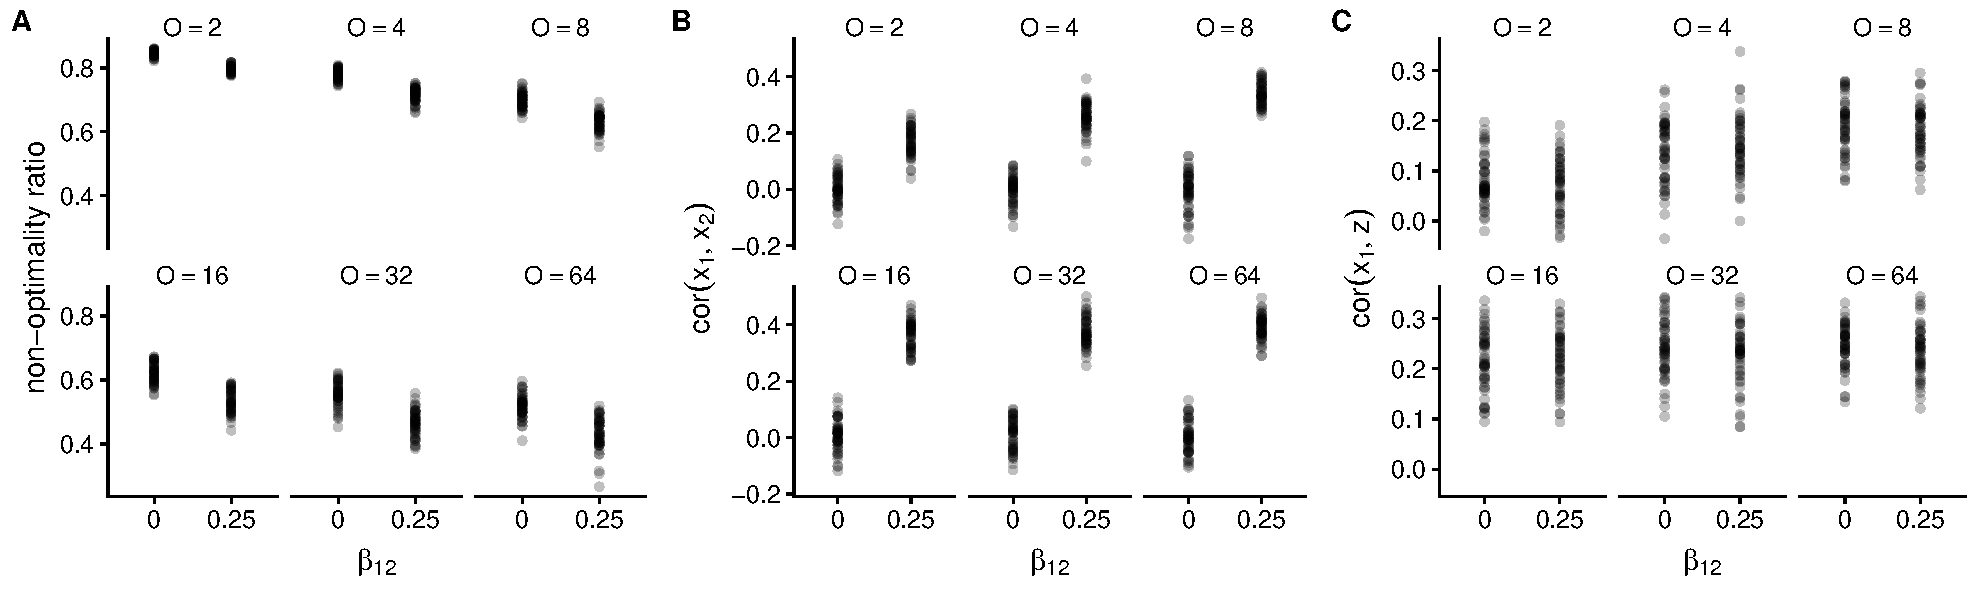
\includegraphics[width=450px]{figure-latex/sample_descriptives.pdf}
\caption[Calibration of Simulated Samples]{\label{calibration} The figure shows the value of the correlation between $\mathbf{x_1}$ and $\mathbf{x_2}$ (Panel A), the correlation between $\mathbf{x_1}$ and $\mathbf{z}$ (Panel B), and the non-optimality ratio (Panel C),  for 100 samples for 6 different levels (2, 4, 8, 16, 32, 64) of the optimality parameter, $O$. The complimentarity effect is either present ($\beta_{12} = 0.25$) or absent ($\beta_{12} = 0$). The decreasing marginal costs are set as $\delta_1 = \delta_2 = 1$. The effect of the environmental variable only affects one of the choices
($\gamma_1 = .33, \gamma_2 = 0$). Lastly, the unobserved variation parameters are set at $\sigma_{\epsilon_1} = \sigma_{\epsilon_2} = \sigma_{\nu} = 1.$}
\end{figure}

\subsection{Type I Error and Power}
In the next section, we will compare the type I error rate and power of the different statistical approaches when varying the optimality parameter, $O$. Because the accounting literature is concerned with testing the hypothesis that there is a (no) complementarity between two management control practices, a focus on error rates and power is appropriate. 

The $\beta_{12}$ coefficients for each specification provide the test for the absence of an interdependency. The simulation generates 1000 samples for each combination of parameters. For each combination, we report the distribution of the t-statistic for the interdependency coefficient and compare it to the traditional cut-off value for the $5\%$ level of significance ($t > 1.97$). We calculate the type I error rate and power of the specifications based on the the p-value of the test to investigate the performance of the demand and performance specifications in more detail. The type I error is the percentage of samples with no complementarity where the p-value is lower than $0.05$. The power is the percentage of samples with a real effect where the p-value is lower than $0.05$ and the estimated coefficient is positive.\footnote{An important caveat is that the power of a study will also be influenced by the size of the effect, measurement error, random variation, and the number of observations in the study. In the simulations, we assumed a fixed effect ($\beta_{12} = 0.25$), no measurement error, fixed the parameters that control random variation, $\sigma_{\epsilon_1}$, $\sigma_{\epsilon_2}$, and $\sigma_{\nu}$, and the number of observations per sample. As a result, the absolute percentages in the results should be interpreted with caution. This study is mainly interested in the relative differences between specifications.}

\section{Results}
\subsection{Performance and Demand Function
Approach}\label{performance-and-demand-function-approach}

In the main results section, we compare the type I error rate and power of the different statistical approaches when varying the optimality parameter, $O$, under variations to the baseline scenario. Figure \ref{main} shows a boxplot for the distribution of t-statistic for each type of test and each combination of parameters. The dot of the boxplot shows the median t-statistic of the 1000 samples, the gap between the whiskers shows the interquartile range, and the whiskers show the minimum and maximum t-statistic. Each boxplot can be compared to the zero line and the dotted lines representing a $95\%$ confidence interval around a null effect. When $\beta_{12} = 0$, we expect the distribution of the t-statistic to be centered on $0$ and $95\%$ of the distribution to be between the two dotted lines. When the distribution is not centered on $0$, the test is biased. When the distribution is too wide, the test reports too many significant interdependencies in the absence of a true effect. When $\beta_{12} = 0.25$, we expect the distribution of the t-statistic to be above the dotted lines because it shows that the test reliably reports a significant positive interdependency.

Figure \ref{main} shows that the demand approach, the theoretically appropriate \emph{performance 1} and the \emph{performance 2} specification have an average t-static close to 0 in the absence of an interdependency. The figure also reveals the basic trade-off between the demand approach and the performance approach: with low levels of optimality the performance function is more likely to detect a true complementarity effect while the demand function is more likely to detect a true complementarity effect with high levels of optimality \citep{grabner_management_2013, aral_three-way_2012, johansson_testing_2018}. Interestingly, even at relatively low levels of optimality, $O = 4$, the demand approach has similar power to the \emph{performance 1} approach. Figure \ref{calibration} shows that with $O=4$ the optimality condition can at best explain $40\%$ of the variation in the distance between the observed level of the practices and the optimal level of the practices. That is, if firms avoid the worst possible combinations of management accounting practices, the demand approach is more likely to detect a true effect.

The \emph{performance 2} specification without the quadratic terms fares worse than the \emph{performance 1} specification at lower optimality levels. The omission of the quadratic terms does not bias the estimate of a complementarity in the absence of the complementarity ($\beta_{12} = 0$) but it decreases the ability of the \emph{performance} specification to detect a real interdependency ($\beta_{12} = 0.25$) at lower levels of optimality. Because the omitted variable bias inflates the complementarity with a factor proportional to the correlation between $x_1$ and $x_2$, the \emph{performance 2} specification has more power to detect a real interdependency at higher levels of optimality. In effect, the bias in \emph{performance 2} picks up the effect of the demand specification.

\begin{figure}
\centerfloat
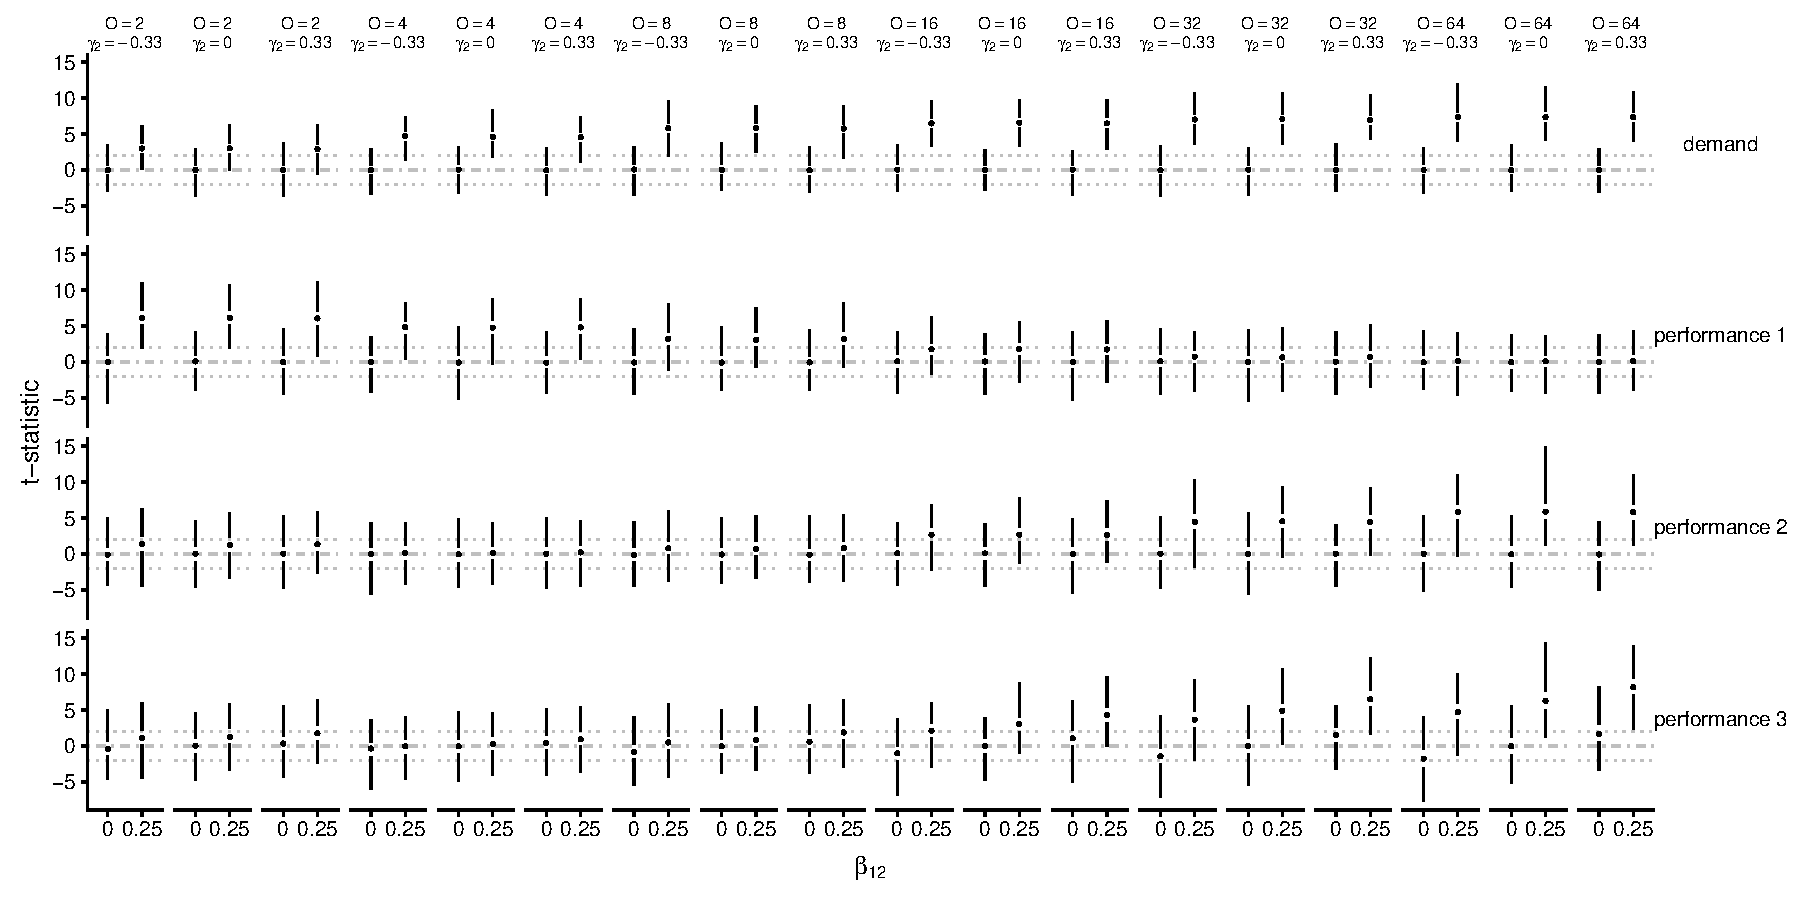
\includegraphics[width=600px]{figure-latex/main_plot.pdf}
\caption[Error Rate and Power of Demand and Performance Specification]
{\label{main} t-static of the performance and demand approach to test
for complementarities when there is a complementarity effect ($\beta_{12} = .25$)
or a null ($\beta_{12} = 0$). The boxplots represent the median (the dot) the
interquartile range (the gap), and the minimum and maximum (the whiskers). $O$
is varied between 2, 4, 8, 16, 32, and 64. The effect of the environmental
variable, $\mathbf{z}$, on the second choice is either absent 
($\gamma_1 = .33,  \gamma_2 = 0$), positive ($\gamma_1 = \gamma_2 = .33$), or negative ($\gamma_1 = .33$ and $\gamma_2 = -.33$).}
\end{figure}


The \emph{performance 3}  specification fares worse than all other specifications. The omission of the interaction terms \(\mathbf{x_1z}\) and \(\mathbf{x_2z}\) biases the estimate of the interdependency when $\gamma_1 \gamma_2 \neq 0$. The bias can be easily seen in Figure \ref{main}. The distribution of t-statistics for the no complementarity datasets no longer centers on $0$ when the environmental factor has a contingency effect on the performance of both practices and the bias increases with higher levels of optimality. The bias is negative when $\gamma_2$ is negative and positive when $\gamma_2$ is positive.  The latter results shows that the most commonly used performance specification currently used in the management accounting literature is inappropriate to test for interdependencies in an observational sample.

\begin{table}[ht]
\centering
\begingroup\footnotesize
\begin{tabular}{lrlrrrrrr}
  \hline
specification & $\gamma_2$ & statistic & 2 & 4 & 8 & 16 & 32 & 64 \\ 
  \hline
demand & -0.33 & type I & 0.05 & 0.05 & 0.05 & 0.04 & 0.04 & 0.05 \\ 
  demand & 0.00 & type I & 0.05 & 0.04 & 0.05 & 0.04 & 0.04 & 0.04 \\ 
  demand & 0.33 & type I & 0.04 & 0.04 & 0.05 & 0.04 & 0.05 & 0.04 \\ 
  performance~1 & -0.33 & type I & 0.17 & 0.14 & 0.18 & 0.16 & 0.15 & 0.14 \\ 
  performance~1 & 0.00 & type I & 0.16 & 0.17 & 0.17 & 0.15 & 0.13 & 0.15 \\ 
  performance~1 & 0.33 & type I & 0.16 & 0.15 & 0.15 & 0.15 & 0.15 & 0.12 \\ 
  performance~2 & -0.33 & type I & 0.20 & 0.19 & 0.18 & 0.16 & 0.21 & 0.22 \\ 
  performance~2 & 0.00 & type I & 0.21 & 0.20 & 0.18 & 0.15 & 0.18 & 0.22 \\ 
  performance~2 & 0.33 & type I & 0.19 & 0.19 & 0.17 & 0.16 & 0.20 & 0.22 \\ 
  performance~3 & -0.33 & type I & 0.21 & 0.20 & 0.22 & 0.30 & 0.40 & 0.48 \\ 
  performance~3 & 0.00 & type I & 0.20 & 0.20 & 0.18 & 0.16 & 0.19 & 0.25 \\ 
  performance~3 & 0.33 & type I & 0.20 & 0.19 & 0.21 & 0.28 & 0.39 & 0.47 \\ 
  demand & -0.33 & power & 0.84 & 1.00 & 1.00 & 1.00 & 1.00 & 1.00 \\ 
  demand & 0.00 & power & 0.84 & 1.00 & 1.00 & 1.00 & 1.00 & 1.00 \\ 
  demand & 0.33 & power & 0.81 & 1.00 & 1.00 & 1.00 & 1.00 & 1.00 \\ 
  performance~1 & -0.33 & power & 1.00 & 0.98 & 0.82 & 0.43 & 0.16 & 0.06 \\ 
  performance~1 & 0.00 & power & 1.00 & 0.98 & 0.82 & 0.43 & 0.19 & 0.07 \\ 
  performance~1 & 0.33 & power & 1.00 & 0.98 & 0.82 & 0.41 & 0.15 & 0.07 \\ 
  performance~2 & -0.33 & power & 0.37 & 0.10 & 0.20 & 0.70 & 0.95 & 0.99 \\ 
  performance~2 & 0.00 & power & 0.32 & 0.10 & 0.22 & 0.69 & 0.96 & 0.99 \\ 
  performance~2 & 0.33 & power & 0.36 & 0.09 & 0.21 & 0.67 & 0.96 & 0.99 \\ 
  performance~3 & -0.33 & power & 0.31 & 0.07 & 0.14 & 0.55 & 0.85 & 0.94 \\ 
  performance~3 & 0.00 & power & 0.34 & 0.12 & 0.27 & 0.76 & 0.97 & 0.99 \\ 
  performance~3 & 0.33 & power & 0.45 & 0.20 & 0.50 & 0.92 & 1.00 & 1.00 \\ 
   \hline
\end{tabular}
\endgroup
\caption{Type I error rates and power for the demand and
             performance function approaches at different levels optimality: 
             2, 4, 8, 16, 32, 64. The parameters are the same as in Figure 
             \ref{basic}.} 
\label{basic-error}
\end{table}


To evaluate the demand and performance specifications in more detail, we report the type I error rate and power of the specifications in Table \ref{main-table}. Under the parameters in the simulation study, the \emph{demand} approach has type I error rates slightly below or equal to the nominal value of $0.05$. This means that the number of false positives are consistent with the nominal p-value of $5\%$. The theoretically appropriate \emph{performance 1} specification tends to have more elevated error rates, two to three times higher than the \emph{demand} specification. The most worrying results are for the \emph{performance 2} and \emph{3} specification. Dropping the quadratic effects increases the error rates in the \emph{performance 2} specification to around $.20$, four times the nominal error rate. The most commonly used specification in the literature, \emph{performance 3}, has even higher type I error rates that increase with higher levels of optimality and when the environmental factor has a contingency effect on both practices. The latter omitted variables lead to a bias in the estimated coefficient for the interdependency and thus the t-statistic. In conclusion, with the parameters in the simulation study only the \emph{demand} specification rejects the null hypothesis at nominal $5\%$ level of significance. The theoretically derived \emph{performance 1} specification has elevated error rates, and the two other performance specifications are even more vulnerable to false positives.

The results for the power of the different specifications shows that the trade-off between the demand specification and the performance specification is a second order problem. Both the \emph{demand} and the \emph{performance 1} specification are able to detect a true interdependency with more than $80\%$ probability for low to medium levels of optimality. However, the \emph{demand} specification is more likely to detect a true effect at higher levels of optimality. The \emph{performance 3} is not able to detect the true interdependency for most of the parameter space under investigation and if it does it comes at the cost of high type I error rates.

One way to interpret this result is to think about how a reader should react when observing a study with a significant positive interaction \(\mathbf{x_1 x_2}\). To demonstrate the problems with the \emph{3} specification, we provide one dramatic example for \(O = 4\) and \(\gamma_2 = 0.33\). If we assume that a priori, we are indifferent between a null effect and a true interdependency of \(\beta_{12} = 0.25\), and we observe one study that reports a significant positive interaction \(\mathbf{x_{1} x_{2}}\), the study is more likely to be from a sample where the null holds than from a sample where there is a true interdependency!

\subsection{Parameter Variations}\label{parameter-variations}

In this section, we explore the robustness of the above conclusions to variations in the parameters of the objective functions. Given the large number of possible variations, we restrict ourselves to theoretically driven comparisons.

\subsubsection{Performance Variation}\label{performance-variation}

We first investigate whether increases in the variance of performance, $\sigma_{\nu}$, change the conclusions. The first effect of increasing the variance is that it decreases the importance of the management practices for performance which decreases the power of the performance specification. The second effect follows from the first. When the management practices are less important, the level of optimality effects are less pronounced, and the correlations between $\mathbf{x_1}$, $\mathbf{x_2}$, and $\mathbf{z}$ are weaker, which in turn decreases the power of the demand specification and the omitted correlated variable bias in the \emph{performance 2} and \emph{performance 3} specification.

To investigate the role of $\sigma_{\nu}$, we vary the parameter between 1, 2, and 4 while keeping the other parameters the same as in Figure \ref{main}. For clarity of exposition, we limit the number of optimality variations ($O = 2, 8, 32$) and the number of variations of the contingency effect $\mathbf{x_2 z}$ ($\gamma_2 = -.33, .33$).

\begin{figure}
\centerfloat
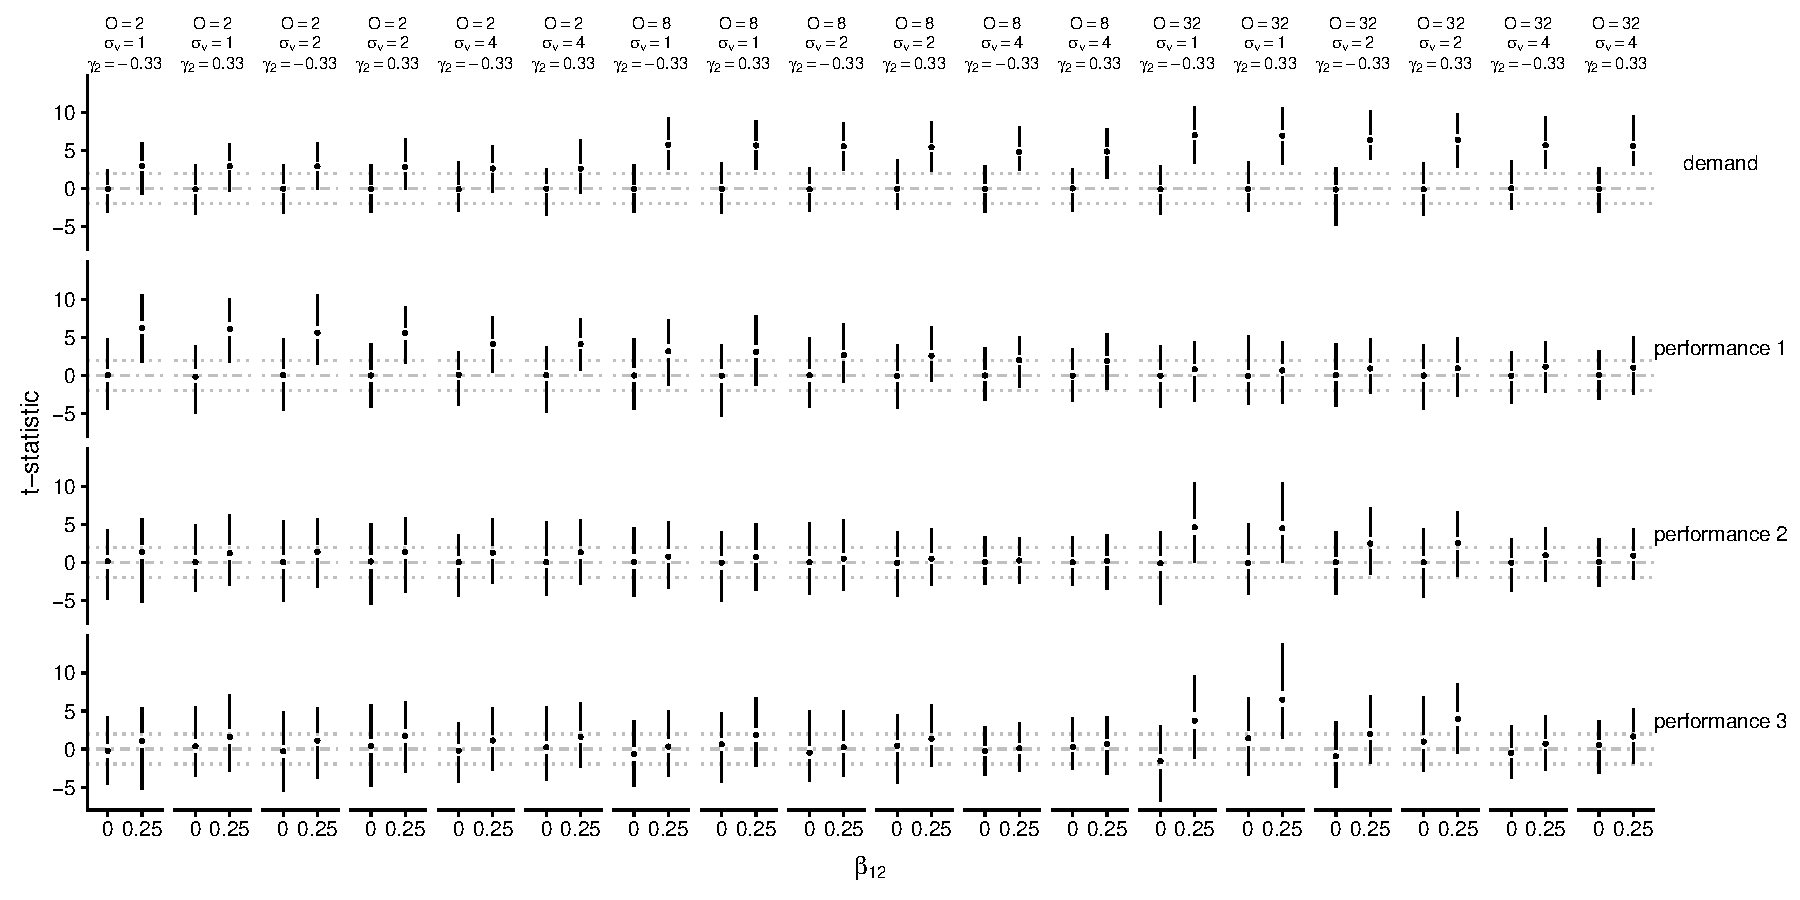
\includegraphics[width=600px]{figure-latex/noise_plot.pdf}
\caption[Error Rate and Power with Increasing Levels of Variability in Performance]
{\label{noise} t-static of the performance and demand approach to test
for complementarities when there is a complementarity effect ($\beta_{12} = .25$)
or a null ($\beta_{12} = 0$). The boxplots represent the median (the dot) the
interquartile range (the gap), and the minimum and maximum (the whiskers). $O$
is varied between 2, 8, 32. The effect of the environmental
variable, $\mathbf{z}$, on the second choice is either positive
($\gamma_1 = \gamma_2 = .33$), or negative ($\gamma_1 = .5$ and $\gamma_2 = -.33$).}
\end{figure}

\begin{table}[ht]
\centering
\begingroup\footnotesize
\begin{tabular}{lrlrrr}
  \hline
specification & $\gamma_2$ & statistic & 2 & 8 & 32 \\ 
  \hline
demand & -0.33 & type I & 0.04 & 0.05 & 0.04 \\ 
  demand & 0.33 & type I & 0.05 & 0.05 & 0.05 \\ 
  performance~1 & -0.33 & type I & 0.09 & 0.06 & 0.06 \\ 
  performance~1 & 0.33 & type I & 0.08 & 0.06 & 0.07 \\ 
  performance~2 & -0.33 & type I & 0.12 & 0.07 & 0.07 \\ 
  performance~2 & 0.33 & type I & 0.13 & 0.07 & 0.07 \\ 
  performance~3 & -0.33 & type I & 0.12 & 0.09 & 0.10 \\ 
  performance~3 & 0.33 & type I & 0.14 & 0.08 & 0.11 \\ 
  demand & -0.33 & power & 0.75 & 1.00 & 1.00 \\ 
  demand & 0.33 & power & 0.75 & 1.00 & 1.00 \\ 
  performance~1 & -0.33 & power & 0.98 & 0.53 & 0.20 \\ 
  performance~1 & 0.33 & power & 0.97 & 0.49 & 0.17 \\ 
  performance~2 & -0.33 & power & 0.30 & 0.06 & 0.16 \\ 
  performance~2 & 0.33 & power & 0.32 & 0.05 & 0.14 \\ 
  performance~3 & -0.33 & power & 0.25 & 0.04 & 0.12 \\ 
  performance~3 & 0.33 & power & 0.39 & 0.11 & 0.37 \\ 
   \hline
\end{tabular}
\endgroup
\caption{Type I error rates and power for the demand and
             performance specifications at different levels optimality: 
             2, 8, 32. The parameters are the same as in Figure \ref{noise}.
             Only the results for $\sigma{nu} = 4$ are reported} 
\label{noise-table}
\end{table}


The results in Figure \ref{noise} and Table \ref{noise-table} are qualitatively the same as the results in Figure \ref{main} and Table \ref{main-table}. The \emph{demand}, the \emph{performance 1}, and the \emph{performance 2} specification are unbiased and the \emph{demand} specification has false positive rates below or close to the nominal rates while the \emph{performance 1} specification has elevated type I error rates. The \emph{performance 2} and \emph{performance 3} specification exhibit the same problem as before, elevated false positive rates as the result of omitted correlated variables. The increase in unobserved performance variation does lessen the impact of the bias.

More importantly, in the presence of an interdependency, the increase in performance variance hardly effects the power of the \emph{demand} specification. At all but the lowest level of optimality, the \emph{demand} specification correctly identifies the interdependency for every simulated sample with a real interdependency although the t-statistics decrease with higher performance variance. The drop-off in the t-statistic is steeper for the \emph{performance 1} specification to the extent that power drops to around \(20\%\) when \(O = 32\) and \(\sigma_{\nu} = 4\). In summary, these results indicate that the major impact of increasing the performance variance is to decrease the power of the performance specifications and only to a lesser extent decrease the effect of the level of optimality, $O$ on the power of the demand specification and the omitted variable bias.

\subsubsection{Marginal Costs}\label{marginal-cost}
 
In this section, we vary the size of the increase in marginal costs, $\delta_1 = \delta_2$. We keep the parameters equal for both management control practices but they become smaller in size. There are two consequences of lowering the increase in marginal costs. First, the bias from omitting the quadratic terms is smaller. Second, decreasing $\delta_1 = \delta_2$ also increases the importance of the complementarity between the management control practices.  In the baseline scenario, we used $\delta_1 = \delta_2 = 1$. In this section, we compare the baseline scenario to two other values $0.25$ and $0$. $\delta_1 = \delta = .25$ is the largest value for which the parameters violates the second-order optimality condition $\beta_{12} < \sqrt{\delta_1 \delta_2}$. The extreme case is when $\delta_1 = \delta_2 = 0$ which may impede the inference by the \emph{demand} specification even further. When the second-order optimality condition is violated, the optimal level for the practices will cluster towards 5 and -5 and away from  0. 

Figure \ref{delta} and Table \ref{delta-table} report the type I error rate and power of the different specifications for samples of firms with slowly increasing ($\delta_i = .25$) or fixed marginal costs ($\delta_i = 0$). Because, the results showed no trends for different values of $\gamma_2$, we aggregated the results over all values of $\gamma_2$ in the table. The \emph{demand} approach suffers from slightly elevated false positives when the marginal costs of the choices are constant or only increasing slowly. Nevertheless, the power of the \emph{demand approach} is generally better for all but the lowest level of optimality and the \emph{performance 1} approach suffers from steep decreases in power with higher levels of optimality.

\begin{figure}
\centerfloat
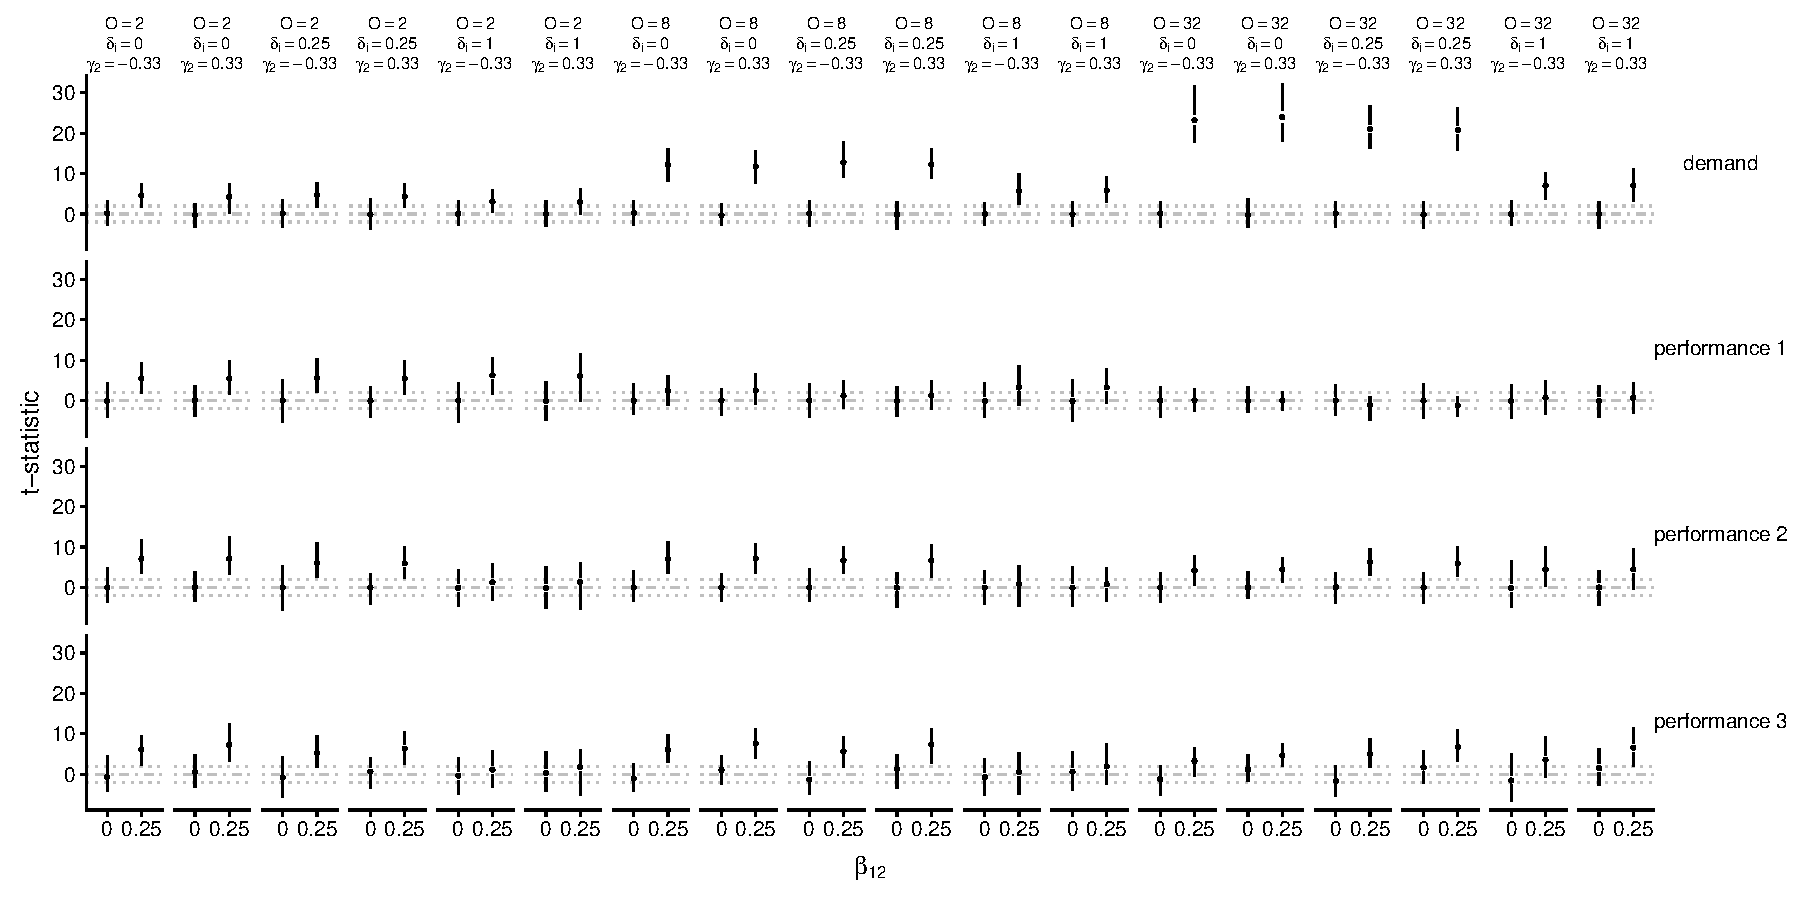
\includegraphics[width=600px]{figure-latex/delta_plot.pdf}
\caption[The Error Rate and Power with Different Levels of Marginal Costs]
{\label{delta} t-static of the performance and demand approach to test
for complementarities when there is a complementarity effect ($\beta_{12} = .5$)
or a null ($\beta_{12} = 0$). The boxplots represent the median (the dot) the
interquartile range (the gap), and the minimum and maximum (the whiskers). $N$
is varied between 2, 8, 32. The effect of the environmental
variable, $\mathbf{z}$, on the second choice is either positive
($\gamma_1 = \gamma_2 = .33$), or negative ($\gamma_1 = .33$ and $\gamma_2 = -.33$).
The increasing marginal costs varied between $\delta_1 = \delta_2 = 0, .25, 1$}
\end{figure}

\begin{table}[ht]
\centering
\begingroup\footnotesize
\begin{tabular}{lrrlrrr}
  \hline
specification & $\gamma_2$ & $\delta_i$ & statistic & 2 & 8 & 32 \\ 
  \hline
demand & 0.33 & 0.00 & type I & 0.06 & 0.06 & 0.04 \\ 
  demand & 0.33 & 0.25 & type I & 0.06 & 0.05 & 0.05 \\ 
  demand & 0.33 & 1.00 & type I & 0.04 & 0.05 & 0.05 \\ 
  performance~1 & 0.33 & 0.00 & type I & 0.11 & 0.08 & 0.07 \\ 
  performance~1 & 0.33 & 0.25 & type I & 0.13 & 0.09 & 0.11 \\ 
  performance~1 & 0.33 & 1.00 & type I & 0.14 & 0.16 & 0.13 \\ 
  demand & 0.33 & 0.00 & power & 0.99 & 1.00 & 1.00 \\ 
  demand & 0.33 & 0.25 & power & 1.00 & 1.00 & 1.00 \\ 
  demand & 0.33 & 1.00 & power & 0.84 & 1.00 & 1.00 \\ 
  performance~1 & 0.33 & 0.00 & power & 1.00 & 0.74 & 0.01 \\ 
  performance~1 & 0.33 & 0.25 & power & 1.00 & 0.24 & 0.00 \\ 
  performance~1 & 0.33 & 1.00 & power & 1.00 & 0.83 & 0.16 \\ 
   \hline
\end{tabular}
\endgroup
\caption{Type I error rates and power for the \emph{demand} and
             \emph{performance 1} specification at different levels optimality: 
             2, 8, 32. The parameters are the same as in Figure \ref{delta}.
             Only the results for $\gamma_{2} = 0.33$ are reported} 
\label{delta-table}
\end{table}


\subsubsection{Binary Practices}

An alternative approach to measure accounting practices with fixed or decreasing marginal costs is to treat them as binary decisions because the optimal decision will either be to use the practice to its full extent or not use it at all. When the accounting practices are binary, the quadratic terms in the \emph{performance 1} specification are no longer identified. Hence, we will compare the \emph{demand} with the \emph{performance 2} specification. In the \emph{demand} specification, we have to take into account that the dependent variable is now a binary outcome. Hence, we compare the linear probability model we have used so far, to the logit and probit estimates of the same specification.  

We simulate new samples for the parameters in the main analysis and with the following levels of optimality: 2, 4, 8, 16. The most important change in algorithm \eqref{eq:firm-simulation} is that we generate the accounting choices, $x_i^o$, no longer from a uniform distribution but let them be $-1$ and $1$ with equal probability and we set the parameters $\delta_1$ and $\delta_2$ equal to $0$.

The results are shown in Table \ref{discrete-table}. Because, the results showed no trends for different values of $\gamma_2$, we aggregated the results over all values of $\gamma_2$. All specifications have similar and acceptable Type I error rates. In this specific case, the \emph{performance 2} specification does not suffer from elevated Type I error rates. The power of the tests is lower for all tests compared to the same results in Table \ref{main-table} for the continuous accounting practices. As before, we find that at all but the lowest level of optimality, the \emph{demand} specification has more power to detect a true effect, independent of the functional form used to estimate the complementarity. With binary practices, we reach the same conclusion as before that the demand specification is superior to the performance specification as long as firms avoid dysfunctional accounting systems. 

\begin{table}[ht]
\centering
\begingroup\footnotesize
\begin{tabular}{llrrrr}
  \hline
specification & statistic & 2 & 4 & 8 & 16 \\ 
  \hline
demand & type I & 0.06 & 0.06 & 0.05 & 0.05 \\ 
  logit & type I & 0.06 & 0.06 & 0.05 & 0.05 \\ 
  performance~2 & type I & 0.06 & 0.05 & 0.05 & 0.05 \\ 
  probit & type I & 0.06 & 0.06 & 0.05 & 0.05 \\ 
  demand & power & 0.27 & 0.72 & 0.96 & 1.00 \\ 
  logit & power & 0.27 & 0.72 & 0.96 & 1.00 \\ 
  performance~2 & power & 0.52 & 0.44 & 0.23 & 0.09 \\ 
  probit & power & 0.28 & 0.72 & 0.96 & 0.99 \\ 
   \hline
\end{tabular}
\endgroup
\caption{Type I error rates and power for the demand and 
  performance specifications at different levels optimality: 2, 
  4, 8, 16. The results are aggregated over the parameter values 
  of $\gamma_2$ (-0.33, 0, 0.33).} 
\label{discrete-table}
\end{table}


% \subsubsection{Asymmetrically increasing marginal
% costs}\label{asymmetrically-increasing-marginal-costs}
% 
% The next variation we investigate are changes in the ratio
% \(\frac{\delta_1}{\delta_2}\) while keeping \(\delta_1 \delta_2 = 1\).
% This means that costs are increasing faster for one practice than for
% the other. The ratio affects the conditional correlation only through
% the parameter, \(\Delta\) (see equation \eqref{eq:conditional}). When
% \(\delta_1\) and \(\delta_2\) are more different, \(\Delta\) increases,
% and \(|\rho^*_c|\) gets closer to \(1\). In addition, as can be seen
% from equation \eqref{eq:demand2}, the standard deviation of
% \(\mathbf{x_1}\) (\(\mathbf{x_2}\)) increases when \(\delta_2\)
% (\(\delta_1\)) increases and vice versa. Both effects, can be seen in
% Figure \ref{scatter-delta} for the following values of
% \(\delta_1 = \delta_2^{-1}\): \(1/3\), \(1\), and \(3\) \footnote{Equation
%   \eqref{eq:coefficient} shows that the standard deviations of
%   \(\mathbf{x_1}\) and \(\mathbf{x_2}\) also effect the regression
%   estimate \(\beta_{12}^d\). As a result, the conditional correlation
%   and the regression demand specification could be expected to yield
%   different results. The simulation results show that the differences in
%   the t-statistic are merely due to numerical differences. As before,
%   for brevity we only report the results for the \emph{demand}
%   regression specification.}.
% 
% \begin{figure}
% 
% 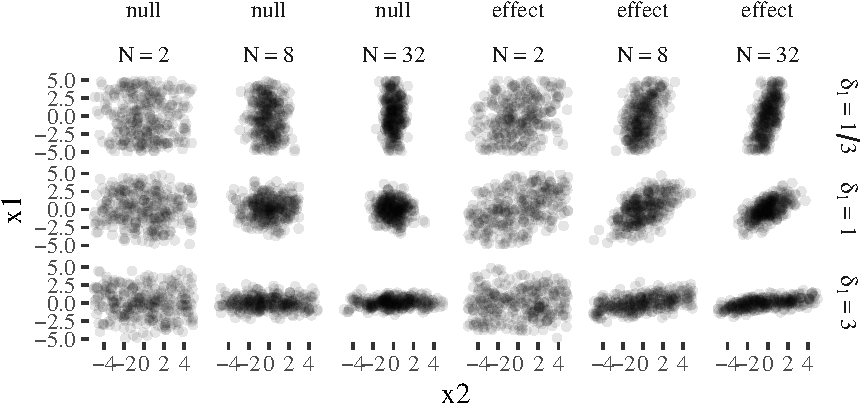
\includegraphics[width=500px]{figure-latex/scatterplot-delta2-1}
% \caption[Distribution of Choices with Asymmetric Marginal Costs]
% {\label{scatter-delta2} Scatter plot of the choices $\mathbf{x_1}$ and
% $\mathbf{x_2}$ for different levels (2, 8, 32) of the optimality parameter, $N$
% with a null interdependency ($\beta_{12} = 0$) or a true effect
% ($\beta_{12} = 0$). The increasing marginal costs are set as
% $\delta_1 = \delta_2^{-1} = 1/3$,$1$, and $3$. The effect of the environmental
% variable only affects one of the choices ($\gamma_1 = .5, \gamma_2 = 0$).
% Lastly, the unobserved variation parameters are set at
% $\sigma_{\epsilon_1} = \sigma_{\epsilon_2} = .5$ and $\sigma_{\nu} = 1.$ }
% \end{figure}
% 
% The simulation results in Figure \ref{scatter-delta2} show that the
% effects of asymmetrically increasing marginal costs is relatively small.
% The general trends for both error rates and power remain the same. The
% \emph{demand} approach has superior error rates and, except for low
% levels of optimality, most power to detect a real effect. The
% \emph{performance 2} and \emph{performance 3} specifications perform
% badly. Nevertheless, asymmetrically increasing marginal costs decrease
% the power of the \emph{demand} specification and increase the power of
% the \emph{performance 1} specification, especially with lower levels of
% optimality.
% 
% \begin{figure}
% 
% 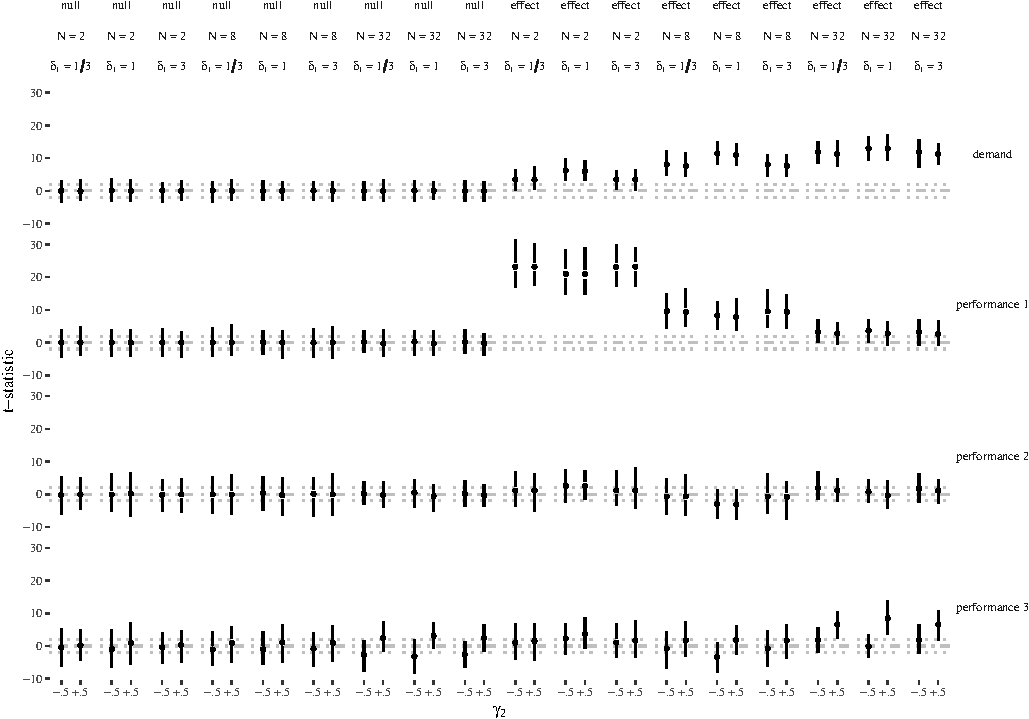
\includegraphics[width=500px]{figure-latex/unnamed-chunk-10-1}
% \caption[Error Rate and Power with Asymmetric with Marginal Costs]
% {\label{delta2} t-static of the performance and demand specification to test
% for complementarities when there is a complementarity effect ($\beta_{12} = .5$)
% or a null ($\beta_{12} = 0$). The boxplots represent the median (the dot) the
% interquartile range (the gap), and the minimum and maximum (the whiskers). $N$
% is varied between 2, 8, 32. The effect of the environmental
% variable, $\mathbf{z}$, on the second choice is either positive
% ($\gamma_1 = \gamma_2 = .5$), or
% negative ($\gamma_1 = .5$ and $\gamma_2 = -.5$). The increasing marginal costs
% are varied at $\delta_1 = \delta_2^{-1} = 1/3, 1$ and $3$}
% \end{figure}

\subsection{Omitted Correlated Variable}

Finally, we investigate to what extent an omitted correlated environmental variable affects our conclusions for the \emph{demand} and \emph{performance 1} specification. The model showed that the omission of a contingency factor that affects the performance of both practices leads to type I errors. To test the vulnerability of the \emph{demand} specification and the \emph{performance 1} specification to spurious correlations in a well designed study, we run the following simulation. We introduce a new unobserved environmental factor \(\mathbf{w}\) that impacts the performance effect of \(\mathbf{x_1}\) with \(\theta_1\) and the performance effect of \(\mathbf{x_2}\) with \(\theta_2\). 

\begin{figure}
\centerfloat
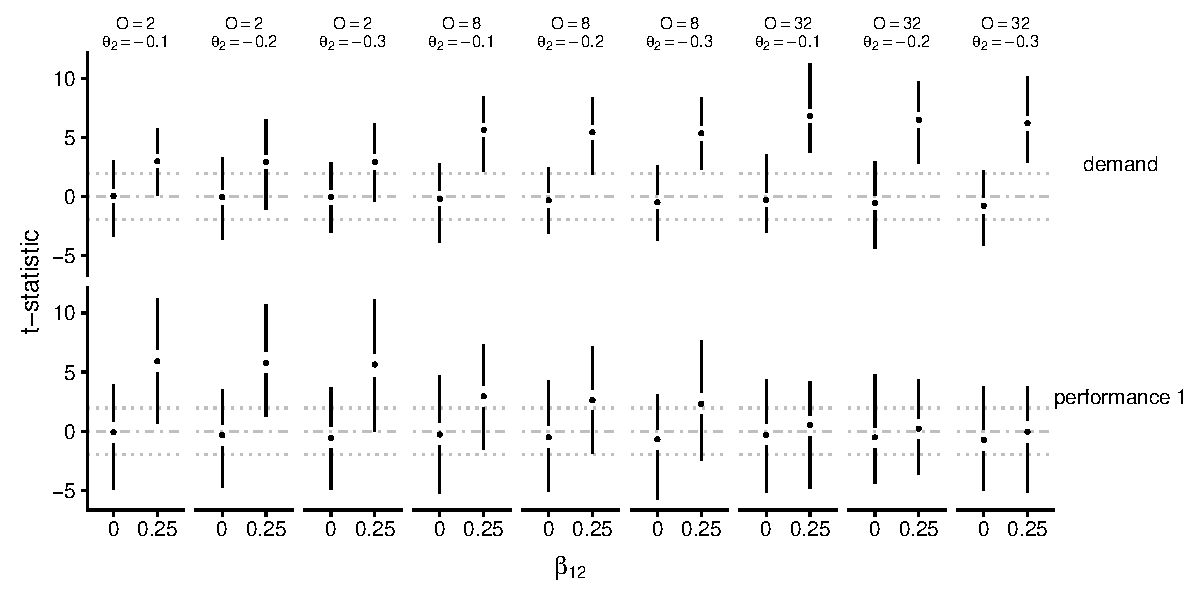
\includegraphics[width=550px]{figure-latex/spurious_plot.pdf}
\caption[Error Rate and Power with Unobserved Environmental Variables]
{\label{spurious} t-static of the performance and demand specification to test
for complementarities when there is complementarity effect ($\beta_{12} = .25$),
or a null effect ($\beta_{12} = 0$). The boxplots represent the median (the dot) the
interquartile range (the gap), and the minimum and maximum (the whiskers). $O$
is varied between 2, 8, 32. The effect of the unobserved environmental variable,
$\mathbf{w}$, on the choices varies from a strong correlation ($\theta_1 = .3$,
$\theta_2 = -.3$), a medium correlation ($\theta_1 = .3$ and $\theta_2 = -.2$),
and a weak correlation ($\theta_1 =.3$, $\theta_2 = -.1$).}
\end{figure}

\begin{table}[ht]
\centering
\begingroup\footnotesize
\begin{tabular}{lrlrrr}
  \hline
specification & $\theta_2$ & statistic & 2 & 8 & 32 \\ 
  \hline
demand & -0.30 & power & 0.84 & 1.00 & 1.00 \\ 
  demand & -0.20 & power & 0.84 & 1.00 & 1.00 \\ 
  demand & -0.10 & power & 0.86 & 1.00 & 1.00 \\ 
  performance~1 & -0.30 & power & 0.99 & 0.63 & 0.06 \\ 
  performance~1 & -0.20 & power & 0.99 & 0.70 & 0.10 \\ 
  performance~1 & -0.10 & power & 1.00 & 0.76 & 0.11 \\ 
  demand & -0.30 & type I & 0.06 & 0.07 & 0.12 \\ 
  demand & -0.20 & type I & 0.05 & 0.05 & 0.08 \\ 
  demand & -0.10 & type I & 0.04 & 0.05 & 0.06 \\ 
  performance~1 & -0.30 & type I & 0.18 & 0.21 & 0.21 \\ 
  performance~1 & -0.20 & type I & 0.17 & 0.20 & 0.18 \\ 
  performance~1 & -0.10 & type I & 0.14 & 0.18 & 0.16 \\ 
   \hline
\end{tabular}
\endgroup
\caption{Type I error rates and power for the \emph{demand} and
             \emph{performance 1} specification at different levels of 
             optimality: 2, 8, 32. The parameters are the same as in Figure 
             \ref{spurious}.} 
\label{spurious-table}
\end{table}


We set the parameters assuming a well designed study that controls for most but not all of the environmental factors affecting the performance of both choices. Based on the 8 studies of the calibration section, we set values for the contingency effect of the unobserved factor that reflect a large ($\theta_1 = 0.3, \theta_2 = -0.3$), medium ($\theta_1 = 0.3, \theta_2 = -0.2$), and small ($\theta_1 = 0.3, \theta_2 = -0.1$) spurious correlation. The methodological literature has long argued an omitted environmental factor will bias the demand specification. We showed above that under the same condition, $\theta_1 \theta_2 \neq 0$, the performance specification will be biased as well. The results of this simulation compare to what extent both specifications are vulnerable to this bias.

The results are reported in Figure \ref{spurious} and Table \ref{spurious-table}. The results are consistent with our previous findings. The \emph{demand} specification has superior type I error rates compared to the \emph{performance 1} specification and at all but the lowest levels of optimality, the \emph{demand} specification has at least the same power to detect a true interdependency as the \emph{performance 1} specification. One important finding is that the \emph{demand} specification becomes vulnerable to the omitted variable bias and higher type I error rates at higher levels of optimality. This effect is most pronounced with the largest spurious correlation (\(\theta_1 = .3\), \(\theta_2 = -.3\)) where we find that in $12\%$ of the simulations with a null effect the \emph{demand} specification reports a significant effect. The finding reinforces that the \emph{demand} specification will only have appropriate type I error rates as part of a well designed study that controls for environmental factors that affect both choices especially when firms adopt the optimal management controls.

\section{Going Forward}

In this section, we use the results to provide guidance for future studies on interdependencies between the management control practices. First, we explain why it will almost always be better to rely on the demand specification in a non-experimental research setting and why researchers should report the results of the demand specification next to the result of the performance specification. Second, we explain how researchers can appropriately control for contingency effects in the performance specifications. Third, we show how the bootstrap and corrections to standard error and degree of freedom calculations can dramatically improve the type I error rates of the performance specification.

\subsection{Reporting the Demand Specification}

Our recommendation applies to studies that test for complementarity with cross sectional data where it is unlikely that firms have almost randomly designed their accounting system. We recommend to always report the demand specification as it will have higher power to detect the complementarity while maintaining appropriate error rates. This recommendation does not put any extra burden on the researcher with respect to data collection because the demand specification does not require additional data.

A researchers might be interested in using the performance specification because they are interested in outcomes that are not the ultimate objective the firm. For instance, researchers are interested which accounting system cause stress in employees\citep{shields_design_2000} and can use the performance specification to investigate this research question. The success of this approach hinges on whether the intermediate outcome (e.g. stress) is related to the final objective (e.g. job performance). In this case, a measure of the intermediate outcome will behave as a noisy measure of the final objective. In the performance specification, the additional noise will be subsumed in the residual term and we showed in Figure \ref{noise} that additional noise hampers the performance specification more than the demand specification. In other words, if the intermediate outcome is related to the final outcome, all the problems with the performance specifications will emerge. 

\subsection{Controlling for Contingency Factors}

One advantage of the performance specification is that it can directly estimate the size of the complementarity in terms of a performance increase. In order to report this estimate, a research should estimate the performance specification with the inclusion of all interactions between the accounting practices, such as delegation and incentives, and contingency factors that affect the performance of the practices, such as environmental uncertainty. When there are a large number of contingency factors that affect both practices, the performance specification has to include a large number of interactions which can yield unstable estimates. We recommend that researchers use a dimension reduction technique such as principal component analysis on the contingency factors to reduce the number of variables and interactions in the regression. This recommendation assumes that the researcher is mainly interested in estimating the complementarity and only includes the contingency factors as control variables.

\subsection{Correcting Type I Errors}

Finally, we address the type I error rates of the performance specification. Even after adjusting for contingency factors, the results show that the performance specification consistently reports higher than nominal false positives. We propose two solutions to this problem. The first one is the bootstrap approach, which relies on repeated resampling of the data to empirically estimate the distribution of the interdependency parameter \citep{efron_computer_2017}. The second one relies on adjustments to the estimates of standard errors and degrees of freedom that are used to calculate t-statistics and p-values \citep{young_improved_2016}.

The bootstrap requires us to run the performance specification repeatedly after resampling the data with replacement. The assumption of the bootstrap is that the data in the sample are representative of the broader population and we can approximate the variation in the population by resampling from our representative sample. For each resampled dataset, we run the performance specification, keep the estimate $\beta_{12}^{p3}$ , and use the distribution of these estimates to decide whether the complementarity is statistically significant. If the $95\%$ confidence interval does not include $0$, the complementarity is considered significant. We use the recommended $2000$ repetitions to get accurate estimates of the confidence interval \citep{efron_computer_2017}. 

We test the type I error rate and the power of the bootstrap for the \emph{performance 1} specification on a subset of the parameters of our main analysis. The computational burden of the bootstrap forces us to limit parameter space. Specifically, we limit the effect of the contingency factor $z$ on $x_2$ to two values ($\gamma_2 = 0.33$ and $\gamma_2 = -0.33$) and we limit the values of the level of optimality to three values ($O=2$, $O=8$, and $O=32$). The results in Table \ref{bootstrap-table} show that the bootstrap reduces the type I error rates of the performance specification considerably and they are close to the nominal $5\%$.  Unfortunately, the improvement in error rates comes at the cost of reduced power to detect a true complementarity.

\begin{table}

\caption{\label{tab:bootstrap-table}Power and Type I Error Rate with Bootstrap}
\centering
\fontsize{9}{11}\selectfont
\begin{threeparttable}
\begin{tabular}[t]{lrrrr}
\toprule
\multicolumn{1}{c}{ } & \multicolumn{1}{c}{ } & \multicolumn{3}{c}{Level of Optimality} \\
\cmidrule(l{3pt}r{3pt}){3-5}
specification & $\gamma_2$ & 2 & 8 & 32\\
\midrule
\addlinespace[0.3em]
\multicolumn{5}{c}{\textbf{Power}}\\
\hspace{1em}performance~1 & -0.33 & 0.99 & 0.68 & 0.09\\
\hspace{1em}performance~1 & 0.33 & 0.99 & 0.65 & 0.08\\
\addlinespace[0.3em]
\multicolumn{5}{c}{\textbf{Type I}}\\
\hspace{1em}performance~1 & -0.33 & 0.06 & 0.07 & 0.06\\
\hspace{1em}performance~1 & 0.33 & 0.05 & 0.07 & 0.06\\
\bottomrule
\end{tabular}
\begin{tablenotes}
\item \textit{Note: } 
\item Type I error rates and power for the 
  \emph{performance 1} specification at different levels of optimality:
  2, 8, 32. $\gamma_2$ is set at either $-0.33$ and $0.33$. 
  The other parameters are the same as in Figure \ref{main}.
\end{tablenotes}
\end{threeparttable}
\end{table}

\citet{young_improved_2016} proposes a computationally efficient alternative adjustment. The adjustment uses the result that the standard error of a coefficient estimate is expected to be chi-squared distributed when the residuals are normally distributed. \cite{young_improved_2016} proposes an adjustment to the standard errors to allow deviations from normality and account for the possibility of influential outliers. In addition, he proposes a further adjustment to the degrees of freedom of the chi-squared distribution and thus of the t-statistic of the coefficient, to account for the fact that the data does not contain completely independent observations. Recall that one of the problems for the performance specification is that optimally designed accounting systems are completely determined by the contingency factors and firms in the same environment have the same accounting system. In other words, firms in the same environment are not independent from each other. As a result, the adjustments to the standard errors and degrees of freedom are relevant to improve the performance specification.

We rerun the main analysis for the \emph{demand} and \emph{performance 1} specification. Table \ref{nearly-table} reports the type I error rate and power of both specifications with and without the corrections. For ease of exposition, we have aggregated the simulations over the different values of $\gamma_2$. The results show that the corrections almost bring the type I error rates to the nominal level of $5\%$. As with the bootstrap results, this comes at the cost of a decrease in the power to detect a true complementarity.\footnote{The corrected standard errors are $2.8\%$ ($O = 2$) to $1\%$ ($O = 64$) smaller for the demand specification and $34\%$ ($O = 2$) to $25\%$ ($O = 64$) higher for the performance specification. The estimated degrees of freedom are $53\%$ ($O = 2$) to $64\%$ ($O = 64$) smaller for the demand specification and $77\%$ ($O = 2$) to $85\%$ ($O = 64$). The correction of the standard errors have the largest impact on the improvement of the performance specification error rate. In practice, the degree of freedom correction could be as beneficial in smaller samples.}

\begin{table}[ht]
\centering
\begingroup\footnotesize
\begin{tabular}{llrrrrrr}
  \hline
specification & statistic & 2 & 4 & 8 & 16 & 32 & 64 \\ 
  \hline
demand & type I & 0.04 & 0.04 & 0.05 & 0.05 & 0.05 & 0.05 \\ 
  demand corrected & type I & 0.05 & 0.05 & 0.05 & 0.05 & 0.05 & 0.05 \\ 
  performance~1 & type I & 0.16 & 0.16 & 0.15 & 0.16 & 0.14 & 0.14 \\ 
  performance~1 corrected & type I & 0.06 & 0.06 & 0.06 & 0.06 & 0.06 & 0.06 \\ 
  demand & power & 0.85 & 1.00 & 1.00 & 1.00 & 1.00 & 1.00 \\ 
  demand corrected & power & 0.86 & 1.00 & 1.00 & 1.00 & 1.00 & 1.00 \\ 
  performance~1 & power & 1.00 & 0.98 & 0.83 & 0.45 & 0.16 & 0.07 \\ 
  performance~1 corrected & power & 0.99 & 0.93 & 0.66 & 0.29 & 0.09 & 0.03 \\ 
  combined & type I & 0.20 & 0.20 & 0.20 & 0.20 & 0.18 & 0.18 \\ 
  combined corrected & type I & 0.11 & 0.10 & 0.10 & 0.11 & 0.10 & 0.11 \\ 
  combined & power & 1.00 & 1.00 & 1.00 & 1.00 & 1.00 & 1.00 \\ 
  combined corrected & power & 1.00 & 1.00 & 1.00 & 1.00 & 1.00 & 1.00 \\ 
   \hline
\end{tabular}
\endgroup
\caption{Type I error rates and power for the demand and
  performance function specification at different levels optimality:
  2, 4, 8, 16, 32, 64. The parameters are the same as in the main 
  analysis in the Figure \ref{main}.} 
\label{nearly-table}
\end{table}


Because the power and type I error rate of the bootstrap and after corrections is indistinguishable, a researcher can report inference based on the performance specification adjusting the OLS results with either of those methods. The bootstrap approach has the advantage that it is more flexible and applicable to other functional forms and multiple equation models. Most modern statistical packages have the functionality to run bootstrap tests. The corrections to test statistics are generally faster but limited to linear models. STATA users can use the script on Alvyn Young's website\footnote{\url{http://personal.lse.ac.uk/YoungA/}} while R users can use the functions in Appendix \ref{appendix-R}.

\subsection{Combining Performance and Demand Specification}

Because the power of the performance specification decreases with the level of optimality while the power of the demand specification increases, a researcher might be tempted to run both regressions and decide that a complementarity is real if either of the regressions reports a significant effect. We assess this combined strategy in Table \ref{nearly-table}. The results show that independent of the level of optimality the combined approach with and without the correction leads to inflated type I error rates. Further investigation of the results shows that the probability to get a false positive in the demand specification for a given sample is independent of the probability a false positive in the performance specification for the same sample.  Therefore, we recommend that researchers use a significance level of $2.5\%$ for each test to keep the Type I error rate at $5\%$ when combining the demand specification and the performance specification. Untabulated simulation results show that this strategy contains the overall Type I error rate to the nominal $5\%$.

\section{Summary and discussion}\label{summary-and-discussion}

This study builds on earlier studies on complementarity theory \citep{milgrom_complementarities_1995, grabner_management_2013}, to provide guidance on how to test for the presence of interdependencies in management control systems. The results of the simulation study show that in most common scenarios the assumptions of optimality should not be the main driver in deciding between the demand or the performance specification. In fact, unless the researchers can make the case that a large number of firms will have a highly dysfunctional management control design, the demand specification should be the preferred statistical method. A straight-forward check on the optimality assumption is to investigate the correlation between the practices and the environmental variables. Non-trivial levels of optimality will induce correlations between management accounting practices and environmental factors when there are contingency effects. Nevertheless, it is important to note that the absence of any correlations does not imply the absence of high levels of optimality as multiple contingency effects can cancel each other out\footnote{An other clarification about the superiority of the demand specification is that it does not imply that the demand function approach provides evidence for high levels of optimality. A statistically significant interdependency effect in the demand specification only implies that firms on average avoid the worst possible management control systems, not that they have on average the optimal control system.}.

When performance data is available, the performance specification can be estimated as an additional test in combination with the demand specification. The performance function approach can be expected to yield acceptable estimates when there is enough performance variation between firms. However, the results of this study show the importance of adequately controlling for environmental factors and potential non-linear performance effects. As far as we know, the current accounting literature does not fully address these correlated omitted variable problems which lead to substantial increases in type I error rates and a loss of power.

The most important weakness of the demand function approach is that it assumes that the performance benefits of management control practices are decreasing with more extensive use. If this second-order condition does not hold, the demand approach might have elevated levels of false positives. We suggest that researchers verify the distribution of the management practices to check whether the second-order condition holds. If one of the management practices has more observations at the extremes of the measurement scale than at the center, the second-order condition might be violated and the results of both the demand and performance specification should be interpreted with care.

TODO: Nod to the solutions in the one but last section

This study has several limitations. Both approaches under investigations have their shortcomings. Our preferred approach, the demand specification, does not allow to directly estimate the performance effect of the interdependency. More sophisticated models are needed to reliably estimate this performance effect. The economics literature has proposed and used a multiple equation model that combines both demand and performance functions \citep{athey_empirical_1998, gentzkow_valuing_2007, kretschmer_competitive_2012, miravete_innovation_2006}. Further research can investigate the appropriateness of these statistical models for the management control setting. An additional advantage of the models is that they can incorporate the effect of unobserved contingency factors and unobserved interdependent practices. A more detailed discussion of these issues goes beyond the scope of this study.

Another limitation of the current study is that the level of optimality is implemented with a naive algorithm that lacks external validity. Better theoretical models of how firms choose management accounting practices can improve upon our understanding of the distribution of management accounting practices and their interdependencies. The approach of Hemmer and Labro \citeyearpar{hemmer_management_2019} is one potential avenue to further explore. They model the firm's choices as decisions under incomplete information with Bayesian updating when more information becomes available. In these models, firms can end up with ex-post sub-optimal management control systems because they lack the appropriate information to choose the optimal system. The parameter governing the lack of information can replace our optimality parameter, \(O\). Further innovations in these models can allow researchers to directly estimate the extent to which firms lack information and choose sub-optimal management control practices.

\pagebreak
 
\appendix
\renewcommand{\theequation}{A.\arabic{equation}}
\setcounter{equation}{0}

\section{General Theory}\label{appendix-general}
% \subsection{General Objective Function}\label{appendix-general}
% 
% We assume that a firm chooses the level of two management accounting practices which depend on one environmental factor. We represent the levels of the management accounting practices as a vector $\mathbf{x}$ and the level of the environmental factors as a vector $\mathbf{z}$. We further assume that the performance, $y$, depends on a factor $\nu$ while the performance effects of each management control practices further depends on a factor $\mathbf{\epsilon}$. In our model, $\mathbf{x}$ and $\mathbf{z}$ are observed by the researcher but $\mathbf{\epsilon}$ and $\nu$ are not. 
% 
% % z and x are column vectors (M x 1) and (N x 1)
% 
% In matrix notation, we can write
% 
% \begin{equation} \label{eq:structural-matrix}
% y = \beta_0 + (\mathbf{\beta_1}^T + \mathbf{z^T} G^T + \mathbf{\epsilon^T})
%      \mathbf{x} + \frac{1}{2}\mathbf{x^T} B \mathbf{x} + \nu
% \end{equation}
% 
% $G$ is a $N \times M$ matrix where each element $\gamma_{nm}$ represents the contingency effect of the observed factor, $z_m$, on practice $x_m$. $B$ is a symmetric $N \times N$ matrix with $\beta_{ij} = \beta_{ji}$ as off-diagonal elements and a vector $-\mathbf{\delta}$ on the diagonal. The off-diagonal elements represent the interdependency between two practices. This follows directly from the definition of an interdependency as the cross derivative of performance to two practices, $\frac{\partial y}{\partial x_i \partial x_j} = .5 \beta_{ij} + .5 \beta_{ji} = \beta_{ij}$. In this paper, we focus on specifications to test the hypothesis that $\beta_{ij} \neq 0$ \footnote{We limit the paper to two-way complementarities for two reasons. First, theory in management control typically does not predict higher order interdependencies (exception \cite{aral_three-way_2012}). Second, the paper's main focus is on the consequences of misspecification in hypothesis tests when the firms in the sample are trying to implement the optimal system but are deviating from it. The problems we identify apply to hypothesis tests for higher order interdependencies. For simplicity, we avoid the complications of testing for higher order interdependencies \citep{carree_note_2011}. For similar reasons, We do not consider contingency effects on the interdependencies \citep{grabner_cost_2016, matejka_balancing_2017}}. For instance, does the effectiveness of incentive contracts depends on the level of delegation for managers \citep{moers_performance_2006}.  The elements of $\mathbf{\delta}$ represent the second derivative of the performance effects of the practices. We assume that all $\delta_n$ are positive which implies increasing marginal costs to the practices  \footnote{$\mathbf{\delta} > 0$ is also a mathematical representation of decreasing marginal returns or a combination of decreasing marginal returns and increasing marginal  costs. For simplicity and in line with the specification in \citet{grabner_management_2013}, we interpret $\mathbf{\delta}$ as the parameter of  increasing marginal costs.}. 
% 
% Further, we assume that the elements of $\mathbf{\epsilon}$ and $\nu$ are independent which implies that the model contains all environmental variables and practices that effect the performance of any two practices $x_i$ and $x_j$. The performance function in equation \eqref{eq:structural-matrix} is similar to the the performance function in \citet{kretschmer_competitive_2012} with two exceptions. First, we assume that the values of $x_n$ are continuous while \citet{kretschmer_competitive_2012} allow for binary practices. We return to the issue of binary practices as an extension to the current model. Second, we assume independence of the unobserved factors. We will relax this assumption, when we introduce the problem of omitted correlated variables further in this section. \citet{athey_empirical_1998} discuss the implications of relaxing the independence assumption in more detail. 
% 
% \subsection{Optimal level of practices}
% 
% In observational data, we expect profit maximising firms to try to adopt the optimal level for each practice or that firms with suboptimal management control systems disappear. Therefore, we derive the optimal level for all practices. The quadratic optimisation problem has a standard solution for the performance function in equation \eqref{eq:structural-matrix} under the condition that $-B$ is positive definite. The solution can be written as follows.
% 
% \begin{equation} \label{eq:optimal-matrix}
% \begin{aligned} 
%     \mathbf{\beta_1} + G \mathbf{z} + \mathbf{\epsilon} & = -B \mathbf{x^*} \\
%     - B^{-1} (\mathbf{\beta_1} +  G \mathbf{z} + \mathbf{\epsilon})  & = \mathbf{x^*}
% \end{aligned}
% \end{equation}
% 
% A number of conclusions can be drawn from equation \eqref{eq:optimal-matrix}. First, in this formulation, the optimal level for each practice can be though of coming from a distribution with mean $-B^{-1} (\mathbf{\beta_1} + G \mathbf{z})$ and covariance matrix $-S_{\epsilon} B^{-1} S_{\epsilon}$ where $S_{\epsilon}$ is the a diagonal matrix with the standard deviations $\sigma_e$ on the diagonal. We can set $-B^{-1} = DRD$ where $R$ is a correlation matrix and $D$ is a diagonal matrix with strictly positive values on the diagonal. The partial correlation between the optimal level of two practices, $x^*_i$ and $x^*_j$ is than given by $-\frac{R^{-1}_{ij}}{\sqrt{R^{-1}_{ii} R^{-1}_{jj}}}$. Because $R^{-1} = - DBD$, the partial correlation between the optimal level of two practices conditional on all other practices and environmental factors equals $\beta_{ij}\lambda_{ij}^*$ where $\lambda_{ij}^* > 0$. In short, the interdependency between two practices fully determines the sign of the partial correlation between the optimal level for these practises. In other words, in our set-up interdependencies between two practices imply a conditional correlation between the optimal levels of these practices. 
% 
% Second, the partial correlation between $x^*_i$ and $z_m$ conditional on all other practices and environmental factors equals $\gamma_{im} \zeta_{im}^*$ with $\zeta_{im}^* > 0$. Similar as before the sign of the conditional correlation between the optimal level of a practice and an environmental factor is given by its the contingency effect, $\gamma_{im}$, of the environmental factor on the practice. 
% 
% Third, when we set $x = x^*$ and combine equation \eqref{eq:structural-matrix} and \eqref{eq:optimal-matrix}, we find that performance, $y$, is fully determined by the unknown parameters and the environmental factors and no longer depends on the value of the choices. That is, performance is no longer a function of the level of the practices. 
% 
% Finally, the second order condition that -B is positive definite implies that for every combination of practices, $\delta_i \delta_j - \beta_{ij}^2 > 0$. The intuition behind this condition is that the increase in marginal costs needs to be relatively large so that the interdependency does not dominate the optimal solution. When the second-order condition does not hold, two complementary practices are both expected to be at either \(+\infty\) or \(-\infty\) and one of two substitutes is \(+\infty\) while the other is \(-\infty\). That is, without large enough increases in marginal costs, management control practices are optimally used to their full extent or not at all. In the main analysis of this paper, we will assume that the second-order condition holds when the control practices are continuous. However, one way to get around the second-order condition is to treat the choice to adopt a management control practice as all or nothing decisions. In the next, section we focus our attention on these binary practices. Note that the second-order condition indicates that binary choices are more likely for practices with weakly increasing or fixed marginal costs or strong interdependencies.
% 
% \subsection{Binary Practices}
% 
% With binary practices, the production function simplifies because $x = x^2$. We can set the parameters of decreasing marginal costs to zero, i.e. $\mathbf{\delta} = 0$. $\beta_{ii}$ now captures the increase in performance from adopting practice $x_i$ when no other practices are adopted and in the absence of any contingency effects. We replace $B$ with $B_0$ which has the same off-diagonal elements as $B$ but $0$ on the diagonal. The optimal decision rule for a firm is to adopt a practice $i$ when profit $y$ is higher for $x_i = 1$ than for $x_i = 0$. 
% 
% \begin{equation} \label{eq:condition-binary}
%     \beta_{ii} + \mathbf{z^T} \mathbf{\gamma_i} + \epsilon_i 
%     + \sum^{N}_{k = 1, k \neq i} \beta_{ik} x_k > 0
% \end{equation}
% 
% Similarly, it is optimal for firms to adopt two practices $i$ and $j$ when the performance is higher than the performance compared to (1) adopting none of the practices, (2) adopting only practice $i$, and (3) adopting only practice $j$. 
% 
% \begin{equation} \label{eq:condition-two-binary}
%     \begin{aligned}
%         \beta_{ii} + \mathbf{z^T} \mathbf{\gamma_i} + \epsilon_i
%         + \beta_{jj} + \mathbf{z^T} \mathbf{\gamma_j} + \epsilon_j
%         + \beta_{ij} + \sum^{N}_{k = 1, k \neq i,j} (\beta_{ik} + \beta_{jk}) x _k &> 0 \\
%         \beta_{jj} + \mathbf{z^T} \mathbf{\gamma_j} + \epsilon_j 
%         + \beta_{ij} + \sum^{N}_{k = 1, k \neq i,j} \beta_{jk} x_k &> 0 \\
%         \beta_{ii} + \mathbf{z^T} \mathbf{\gamma_i} + \epsilon_i
%         + \beta_{ij} + \sum^{N}_{k = 1, k \neq i,j} \beta_{ik} x_k &> 0 
%     \end{aligned} 
% \end{equation}
% 
% This line of reasoning can be extended for the necessary inequality conditions for the optimal adoption of $p \leq N$ binary practices. However, we do not need the complete set of conditions to illustrate that the same set of conclusions hold as for the continuous practices. First, whether a practice is optimally adopted depends on the contingency factors. Second, whether two practices are adopted together depends the interdependency parameter $\beta_{ij}$. In the absence of interdependencies, $\beta_{12} = 0$, the second and third condition in equation \eqref{eq:condition-two-binary} simplify to the condition \eqref{eq:condition-binary} and when they are both satisfied, the first condition holds as well. That is, in the absence of an interdependency between practices, the adoption of one practice is not a function of the adoption of the other practice.
% 
% \subsection{Empirical Correlations}
% 
% As explained in the previous section, when firms adopt the optimal practices, $x^*_i$, they are a function of the contingency factors, $z_m$, when $\gamma_{im} \neq 0$ and conditional on all other practices and contingency factors. Similarly, the practices $x^*_i$ and $x^*_j$ are a function of each other conditional on all other environmental factors when $\beta_{ij} \neq 0$. In the remainder of this section, we will work with the more tractable continuous model where the partial correlation is a either $\gamma_{im}$ or $\beta_{ij}$ scaled by a positive factor. The derivations for binary practices depend on additional assumptions about the distribution of the unobservable contingency factors $\epsilon$. Nevertheless, the qualitative conclusions are expected to hold for binary practices and we will test these expectations in the simulation study.
% 
% The strength of the conditional correlation between practices and environmental factors will also depend on the extent to which firms have adopted optimal practices. We assume that the conditional correlation between practices and environmental factors equals $0$ when firms adopt practices in complete ignorance of the optimal level, while the conditional correlation goes to $\gamma_{im}\zeta_{im}^*$ when all firms adopt the optimal level of each practice. Similarly, we assume that the actual observed conditional correlation between two practices will depend on the extent to which firms have adopted the optimal level for each practice. In complete absence of knowledge about the optimal levels, the conditional correlation is assumed to be $0$ while it goes to $\beta_{ij}\lambda_{ij}^*$ when firms adopt the optimal levels. 
% 
% \subsection{Performance Specification.}
% 
% The performance function approach estimates the performance equation \eqref{eq:structural-matrix} directly. With cross-sectional data, the closest approximation to the structural equation is the following regression model where the subscript for each observation is suppressed. 
% 
% \begin{equation*}
%     y = \beta_0^{p1} + \mathbf{\beta_z^{p1^T} z} + (\mathbf{\beta_1^{p1^T}} + \mathbf{z^T} G^{p1^T}) \mathbf{x} + 
%     \frac{1}{2}\mathbf{x^T} B^{p1} \mathbf{x} + \nu^{p1}
% \end{equation*}
% 
% The specification captures all features of the unobserved performance function in equation \eqref{eq:structural-matrix} with the exception of the unobservable heterogeneity in the performance effects of the management choices, $\mathbf{\epsilon}$. Cross-sectional data does not permit estimating the unobservable heterogeneity. In this specification, \(\beta_{ij}^{p1}\) tests for the interdependency between the management accounting practices. We are not aware of any accounting studies using this specification which we label the \emph{performance 1} specification. 
% 
% For binary practices, we can replace $B$ by $B_0$ and effectively drop the quadratic terms, $x_i^2$.  While investigating continuous practices, \citet{bedford_management_2016} follow the above specification as they control appropriately for contingency factors but they drop the quadratic terms in the specification. We call this the \emph{performance 2} specification.
% 
% \begin{equation*}
%     y = \beta_0^{p2} + \mathbf{\beta_z^{p2^T} z} + (\mathbf{\beta_1^{p2}} + \mathbf{z^T} G^{p2}) \mathbf{x} + 
%     \frac{1}{2}\mathbf{x^T} B_0^{p2} \mathbf{x} + \nu^{p2}
% \end{equation*}
% 
% The bulk of the literature follows the third performance specification which also drops the controls for the contingency factors or assumes that all elements of $G$ equal $0$. We call this specification \emph{performance 3}.
% 
% \begin{equation*}
%     y = \beta_0^{p3} + \mathbf{\beta_z^{p3^T} z} + \mathbf{\beta_1^{p3}} \mathbf{x} + 
%     \frac{1}{2}\mathbf{x^T} B_0^{p3} \mathbf{x} + \nu^{p3}
% \end{equation*}
% 
% \subsubsection{Lack of Power}
% 
% In the remainder of this section, we explain the potential problems with these three specifications. All three specifications, will suffer form the well known problem we explained above that performance is no longer a function of the management practices when firms adopt the optimal practices \citep{grabner_management_2013}. With strictly optimal practices, there is no longer information about the practices in the performance variable. The literature advises that for a performance specification to have sufficient power, there need to be a sufficient number of firms that are not adopting the optimal level of the practices \citep{bedford_management_2016, carree_note_2011, hofmann_organizational_2017}. However, the literature has not gone beyond this rule of thumb to investigate how strong the deviations from optimality need to be. Our simulation study will provide an answer to this question.
% 
% \subsubsection{Correlated Omitted Variables}
% 
% In this paper, we identify a second problem with the most popular specification in the literature, \emph{performance 3}, which follows directly from contingency theory. As explained in the previous section, contingency theory implies empirical conditional correlations between environmental factors and practices when firms are not completely ignoring the performance effects of the environmental factors. As a result, when environmental factors are not appropriately controlled for, regression estimates are vulnerable to an omitted correlated variable bias. Because the bias does not require perfectly optimal decisions, and follows directly from contingency theory this problem cannot be easily ignored in a typical management accounting study. More importantly, this bias does not require any interdependencies. In other words, a regression analysis will report a false positive interdependency when the specification does not adequately control for environmental factors. 
% 
% We showed above that the conditional correlations between environmental factors and practices are proportional to the contingency effect, $\gamma_{im}$. As a result, we can write the empirical relation between $\mathbf{z_m}$ and two practices, $x_i$ and $x_j$, as $\mathbf{z_m} = \gamma_{im} \zeta^p_{im} \mathbf{x_i} + \gamma_{jm} \zeta^p_{jm} \mathbf{x_j} + \mathbf{\epsilon_z}$ with all $\zeta^p$'s $>0$ when not all firms are completely ignorant about the optimal levels for the practices.  When the terms associated with the contingency effect are omitted from the production function as in \emph{specification 3}, we can derive the bias on the estimate of $\beta_{ij}$ as follows.
% 
% \begin{align*}
% \gamma_{im} \mathbf{z_m} \mathbf{x_i} + \gamma_{jm} \mathbf{z_m} \mathbf{x_j}
% = \gamma^2_{im} \zeta^p_{im} \mathbf{x_i}^2 + \gamma^2_{jm} \zeta^p_{jm} \mathbf{x_i}^2 
%     + \gamma_{im} \gamma_{jm} (\zeta^p_{im} + \zeta^p_{jm}) \mathbf{x_i x_j} 
%     + \epsilon_z ( \mathbf{x_i} + \mathbf{x_j})\\
% \end{align*}
% Which implies that the estimate $\beta^{p3}_{ij}$ will be biased by $\gamma_{im} \gamma_{jm}(\zeta^p_{im} + \zeta^p_{jm})$. Thus, the interdependency estimate will be biased in a production function specification that does not adequately control for an environmental factor with a contingency effect on both practices, unless firms are ignorant about the optimal levels for each practice. So far, we have argued that the bias will occur with the \emph{performance 3} specification. It is important to note that the other specifications are also vulnerable to this bias if they do not include all interaction terms between practices and environmental factors with contingency effects on at least two of the practices. 
% 
% A similar problem emerges when a specification does not appropriately control for all interdependent practices. We can write the empirical relation between one practice and two other practices as $\mathbf{x_k} = \beta_{ik} \lambda^p_{ik} \mathbf{x_i} + \beta_{jk} \lambda^p_{jk} \mathbf{x_j} + \mathbf{\epsilon_x}$ with all $\lambda^p$'s $>0$ when not all firms are completely ignorant about the optimal levels for the practices. Similar as before, we can show that the estimate of $\beta_{ij}$ will be biased by $\beta_{ik} \beta_{jk} (\lambda^p_{ik} + \lambda^p_{jk})$. More specifically, the bias will manifest when the performance specification omits a practice that is dependent on two other practices and at least some firms take these interdependencies into account when designing an accounting system.
% 
% A special case of the above problem is the omission of the quadratic terms $\delta_i \mathbf{x_i}^2$ where $\mathbf{x_i} =  \beta_{ij} \lambda^p_{ij} \mathbf{x_j} + \mathbf{\epsilon_x}$. As a result, this omission will bias the estimate of $\beta_{ij}$ with $\beta_{ij} 
% \delta_i \lambda^p_{ij}$. Since $\lambda^p_{ij} > 0$, this bias will not change the sign of the estimate but will inflate the estimate with a factor $1 + \delta_i \lambda^p_{ij}$.  This result also implies that the omission will not bias estimates when $\beta_{ij} = 0$. The omission of the quadratic term is the difference between the \emph{performance 1} and \emph{performance 2} specification.
% 
% The empirical and methodological literature has largely ignored the problem of correlated omitted environmental factors and practices in performance specifications. It has been recognized that the demand specification suffers from the bias when two practices are contingent on an unobserved environmental factor or when they are both interdependent with a third practice (see also section \ref{demand-specification}. We show that the performance specifications suffer from the exact same bias in contrast to what has been argued in the methodological literature \citep{carree_note_2011}. 
% 
% The strength of the correlation between practices and environmental factors and thus the extent of the omitted correlated variable bias depend on the extent to which firms have adopted optimal practices ($\lambda$'s and $\zeta$'s). In contrast to the problem of a lack of power, these correlations will manifest, even if not all firms adopt the optimal level for all practices. Our simulation study will investigate the intermediate regime where firms attempt to adopt the optimal level of the practices but do not succeed entirely.
% 
% \subsection{Demand Specification}\label{demand-specification}
% 
% The \emph{demand specification} can take two forms, a regression approach and the conditional correlation approach. In this section, we explain the equivalence between the two approaches. The regression  approach to detect an interdependency between two practices, $x_i$ and $x_j$, uses one of those practices as the dependent variable and the other as independent variable and controls for all other practices and the environmental factors.
% 
% \begin{equation} \label{eq:demand-specification}
% \mathbf{x_i} = \beta_0^d + \beta_{ij}^d \mathbf{x_j} 
% 		+ \sum_{k = 1, k \neq i,j}^N \beta_{ik}^d \mathbf{x_k} 
%         + \sum_{m = 1}^M \gamma_{im}^d \mathbf{z_m}
%         + \mathbf{\epsilon^d}
% \end{equation}
% 
% The regression specification approximates the optimality condition  \eqref{eq:optimal-matrix} where \(\beta^d_{ij}\) is the parameter that estimates the complementarity effect. $\beta_{ij}^d$ is proportional to the  correlation between $\mathbf{x_i}$ and $\mathbf{x_j}$ conditional on all other practices and environmental factors as a result  $\beta^d_{ij} = \beta_{ij} \lambda^d_{ij}$ with $\lambda^d_{ij} > 0$ if at least some firms take into account the interdependency when designing the accounting system. Therefore, a disadvantage of the regression approach is that it cannot directly estimate size of the interdependency.
% 
% The conditional correlation approach estimates the correlation matrix $R = -D^{-1}B^{-1}D^{-1}$ between the practices  conditional on the environmental practices where $D$ is a diagonal matrix. Prior research has used seemingly unrelated regressions and OLS regressions to condition on the environmental practices \citep{Indjejikian2012, matejka_balancing_2017}. Early methodological work argued that the estimated conditional correlation , $R^c_{ij}$, test whether there are any interdependencies in the accounting system involving both $x_i$ and $x_j$ \citep{arora_testing_1996}.  Later empirical work, estimates the partial correlation matrix ${R^c}^{-1}$. Because ${R^c}^{-1}_{ij} = \beta_{ij} \lambda^c_{ij}$ , the partial correlation tests directly for an interdependency between $x_i$ and $x_j$ \citep{Indjejikian2012}. 
% 
% In this study, we are interested in comparing the robustness of different tests whether an interdependency between two practices exists. As we showed above, the partial conditional correlation approach and the regression approach are equivalent in that they estimate the interdependency, $\beta_{ij}$, scaled by a positive factor. In the remainder of the paper, we will explain the problems with the demand specification from the perspective of the regression approach. Those problems equally apply to the conditional correlation approach.  
% 
% \subsubsection{Lack of Power}
% 
% When firms do not take into account the interdependencies and the contingency effects, the empirical correlations will not manifest. A regression estimate $\beta^d_{ij} = \beta_{ij} \lambda^d_{ij}$ results in $\lambda^d_{ij}$ = 0 when no firm takes into account the interdependencies between the practices when designing the accounting system. In the remainder of this study, we consider this an unreasonable  assumption in the absence of a natural experiment for the adoption of both practices, $x_i$ and $x_j$. In the simulation study, we will investigate what happens when we vary the extent to which firms adopt the optimal practices. When firm's system deviate strongly form the optimal accounting system, $\lambda^d_{ij}$ will be small and the demand specification will lack power to detect a real interdependency.
% 
% \subsubsection{Simultaneity Bias}
% 
% Because all practices are jointly determined, this regression model will suffer from simultaneity bias \citep{Chenhall2007} if there are interdependencies between the practices. If $B^{-1}_{ij} \neq 0$, the unobserved environmental factors that affect one practice, $\epsilon_i$, will also affect the other practice, $x_j$. Nevertheless, as we shown above, $\beta^d_{ij} = \beta_{ij} \lambda^d_{ij}$. Thus, the simultaneity bias does not affect the sign of $\beta^d_{ij}$ and the estimate will be 0 when there is no interdependency between the practices. 

% \subsubsection{Correlated Omitted Variables}
% 
% Similar as for the performance specification, we can investigate the impact of omitted environmental factors from the regression model. We can write the omitted environmental factor as $z_m = \zeta_{im}^d \gamma_{mi} \mathbf{x_i} +  \zeta_{jm}^d \gamma_{mj} \mathbf{x_j} + \mathbf{\epsilon_z}$ and the parameters. The omission of the environmental factor will bias the estimate $\beta^d_{ij}$ by $\frac{\zeta^d_{im} \zeta^d_ {jm}\gamma_{im} \gamma_{jm}}{1 - \zeta^d_{im} \gamma_{im}}$. As with the performance specification, we find that the interdependency estimate of the demand specification will be biased when the regression omits an environmental variable with a contingency effect on two practices.
% 
% Similarly, we can investigate the omission of a practice $\mathbf{x_k}$ from the demand specification. With $\mathbf{x_k} = \beta_{ik} \lambda^d_{ik} \mathbf{x_i} + \beta_{jk} \lambda^d_{jk} \mathbf{x_j} + \mathbf{\epsilon_x}$, the bias on the estimate by $\frac{\lambda^d_{ik} \lambda^d_{jk} \beta_{ik} \beta_{jk}}{1 - \lambda^d_{ik} \beta_{ik}}$ . Similar as in the performance specification, the estimate of an interdependency between two practices will be biased when a third practices that depends on both practices is omitted. 
 
\section{Omitted Variable Bias} \label{appendix-omitted}

The bias of omitting the term $\mathbf{x_1 z}$ on the estimate of $\beta^{p3}_{12}$ is given by $\gamma_1 \frac{cov(\widetilde{\mathbf{x_1 x_2}}, \widetilde{\mathbf{x_1 z}})} {var(\widetilde{\mathbf{x_1 z}})}$ where $\widetilde{\mathbf{x_1 x_2}}$ and $\widetilde{\mathbf{x_1 z}}$ are the residual vector of regressing $\mathbf{x1}$, $\mathbf{x2}$, and $\mathbf{z}$ on $\mathbf{x_1 z}$ and $\mathbf{x_1 z}$ respectively \citep{angrist2008mostly,cunningham_causal_2018}. 
Assume that $\mathbf{x1}$, $\mathbf{x2}$, and $\mathbf{z}$ are multivariate standard normal with correlations $r_{12}$, $r_{2z}$, and $r_{1z}$. We can use the \citet{isserlis_formula_1918} formula to derive the covariance between an interaction and one of the variables. 

\begin{align*}
cov(\mathbf{x_1 x_2}, \mathbf{x_1}) &= E(\mathbf{x_1}^2 \mathbf{x_2}) - E(\mathbf{x_1 x_2}) E(\mathbf{x_1}) \\
&= 0 - 0 \\
cov(\mathbf{x_1 x_2}, \mathbf{x_2}) &= 0 \\
cov(\mathbf{x_1 x_2}, \mathbf{z}) &= 0 \\
cov(\mathbf{x_1 z}, \mathbf{x1}) &= 0 \\
cov(\mathbf{x_1 z}, \mathbf{x2}) &= 0 \\
cov(\mathbf{x_1 z}, \mathbf{z}) &= 0 \\
\end{align*}
Where we make use of the fact that the expectation of the product of an odd number of standard normal variables equals 0. In the simplest case, $E(\mathbf{x_1}) =  E(\mathbf{x_2}) = E(\mathbf{z}) = 0$.
As a result,

\begin{equation*}
\frac{cov(\widetilde{\mathbf{x_1 x_2}}, \widetilde{\mathbf{x_1 z}})}{var(\widetilde{\mathbf{x_1 z}})} =
\frac{cov(\mathbf{x_1 x_2}, \mathbf{x_1 z})}{var(\mathbf{x_1 z})} 
\end{equation*}
where 

\begin{align*}
cov(\mathbf{x_1 x_2}, \mathbf{x_1 z}) &= E(\mathbf{x_1}^2 \mathbf{x_2 z }) - E(\mathbf{x_1 x_2}) E(\mathbf{x_1 z}) \\
&= E(\mathbf{x_1}^2) E(\mathbf{x_2 z }) + E(\mathbf{x_1 x_2}) E(\mathbf{x_1 z}) + E(\mathbf{x_1 z}) E(\mathbf{x_1 x_2}) - E(\mathbf{x_1 x_2}) E(\mathbf{x_1 z}) \\
&= E(\mathbf{x_1}^2) E(\mathbf{x_2 z }) + E(\mathbf{x_1 x_2}) E(\mathbf{x_1 z}) \\
&= r_{2z} + r_{12} r_{1z}
\end{align*}
In the last line we make use of the fact that E($\mathbf{x_1^2}) = var(\mathbf{x_1}) = 1$.

\begin{align*}
	var(\mathbf{x_1 z}) &= E(\mathbf{x_1^2 z^2}) - E(\mathbf{x_1 z}) E(\mathbf{x_1 z}) \\
	&= E(\mathbf{x^1}) E(\mathbf{z}) +  E(\mathbf{x_1 z}) E(\mathbf{x_1 z}) + E(\mathbf{x_1 z}) E(\mathbf{x_1 z}) - E(\mathbf{x_1 z}) E(\mathbf{x_1 z}) \\
	&= 1 + r^2_{1z}
\end{align*}
Putting it all together the bias of omitting the term $\mathbf{x_1 z}$ on the estimate of $\beta^{p3}_{12}$ is  $\gamma_1 \frac{r_{2z} + r_{12} r_{1z}}{1 + r^2_{1z}}$

Similarly, the bias of omitting the term $\mathbf{x_1 z}$ on the estimate of $\beta^{p3}_{12}$ is  $\gamma_2 \frac{r_{1z} + r_{12} r_{2z}}{1 + r_{2z}^2}$

The bias of omitting the terms $\mathbf{x_1^2}$ and $\mathbf{x_2^2}$ is respectively $\delta_1 r_{12}$ and $\delta_2 r_{12}$

\section{R Functions Nearly Exact Correction} \label{appendix-R}
\begin{lstlisting}[language=R]
#' Install the sandwich package if necessary
if (!require("sandwich")) install.packages("sandwich")

#' Calculate the nearly exact bias and edf for the HC1 Variance
#' Estimator.
#' @param x design matrix of the regression
#' @param w hypothesis test
nearly_exact <- function(x, w){
  N = nrow(x); k = ncol(x) - 1; c = N / (N - k);
  xx <- solve(crossprod(x))
  M = diag(rep(1, N)) - tcrossprod(x %*% xx, x)
  z = tcrossprod(t(w) %*% xx, x); zz = z %*% t(z); z2 = z^2;
  mu = c/zz * sum(z^2 * diag(M))
  nu = 2 * c^2 / zz^2 * (tcrossprod(z2 %*% M^2, z2))
  edf = 2 * mu^2 / nu
  return(list(mu = as.numeric(mu), edf = as.numeric(edf)))
}

#' Calculate the coefficient table for the nearly
#' exact bias and df correction.
#' @param formula The regression formula as would be used with lm
#' @param data A dataframe
#' @param pdigits Number of digits to round the p-value

lm_nearly <- function(formula, data, pdigits = 4){
  reg <- lm(formula = formula, data = data)
  x <- model.matrix(object = formula, data = data)
  covHC <- sandwich::vcovHC(x = reg, type = "HC1")
  seHC <- sqrt(diag(covHC)); varnames <- names(seHC); 
  coefficients <- data.frame(matrix(nrow = length(varnames), ncol = 6))
  names(coefficients) <- c("variable", "estimate", "se",
                           "t value", "df", "p value")
  coefficients$variable <- varnames
  for (var in varnames){
    hypothesis = I(varnames == var)
    correction <- nearly_exact(x = x, w = hypothesis)
    se = seHC[var] / sqrt(correction$mu)
    stat <- reg$coefficients[var]/se
    coefficients[coefficients$variable == var, 2:6] <- c(
      reg$coefficients[var], se, stat, correction$edf, 
      round(2 * pt(abs(stat), correction$edf, lower.tail = FALSE),
            pdigits)
    )
  }
  return(list(coefficients = coefficients, lm = reg))
}

#' Useage

corrected <- lm_nearly(speed ~ dist, cars)
print(corrected$coefficients, digits = 2)
\end{lstlisting}

% \subsection{Quotes}
% 
% 
% \begin{quote}
% Which {[}specification{]} to use is both a theoretical (assumption of agents as perfectly or boundedly rational) and an empirical (market imperfections, exogenous shocks, experimentation, etc) issue because the likelihood of finding evidence of the former depends on the latter and vice versa (Grabner and Moers, 2013; Gerdin and Greve, 2004). (in Johansson, 2016).
% \end{quote}
% 
% \begin{quote}
% decision makers may not have been sufficiently well informed such that they chose efficiency or output enhancing combinations of practices.
% \citep{carree_note_2011}
% \end{quote}
% 
% Others have argued that the performance specification can be applied ``as long a the populaetion of organizations includes a reasonable number of organizations that takes non-optimal combinations of practice'' \citep{carree_note_2011}.
% 
% About the conditional correlation approach.
% \begin{quote}
% While this approach certainly has intuitive appeal and is easy to implement, it also relies on a strong assumption that the set of conditioning variables is reasonably complete. Without a well-specified reduced form regression, the correlation between the residual (p. 459) terms might not signal complementarity but rather the presence of a third factor that is correlated with the two organizational design choices under consideration. from (Hoffman and van Lent).
% \end{quote}
% 
% \begin{quote}
% This focus is appropriate as the control problems examined in this study (i.e. the alignment of behaviours to the strategic objectives of the firm) are complex and require significant experimentation by top management, particularly in conditions characterized by uncertainty such as the prospector strategic context (Simons, 1995). Hence it is unlikely that firms will be, on average, in an optimal equilibrium. in \citep{bedford_management_2016}
% \end{quote}
% 
\newpage

\bibliographystyle{model5-names.bst}
\bibliography{references2.bib}

\end{document}
